% IE 643 Course Project: Intensive Assessment Report
% Team: Unemployed and Unsupervised
%
% DRAFT. Before submitting, both of us must rewrite every paragraph in our own words
% (the course runs a plagiarism and AI-content check). See README.md in this folder.
% Compile on Overleaf with pdfLaTeX: upload this folder, set report.tex as the main file.

\documentclass[11pt,a4paper]{article}

\usepackage[margin=2.2cm]{geometry}
\usepackage[T1]{fontenc}
\usepackage[utf8]{inputenc}
\usepackage{lmodern}
\usepackage{microtype}
\usepackage{graphicx}
\usepackage{booktabs}
\usepackage{amsmath,amssymb}
\usepackage{xcolor}
\usepackage{enumitem}
\usepackage{caption}
\usepackage{float}
\usepackage[hidelinks]{hyperref}

\graphicspath{{figures/}}
\setlist{itemsep=2pt,topsep=4pt}
\newcommand{\todo}[1]{\textcolor{red}{[TODO: #1]}}

\title{\textbf{Cross-Template Key-Value Field Extraction from Scanned Forms:\\
Generalizing to Form Templates With Zero Same-Template Training Data}\\[6pt]
\large IE 643 Course Project, Intensive Assessment Report}
\author{Team: Unemployed and Unsupervised\\[4pt]
Param Mehta (23b2439) \quad Arjoe Basak (23b1295)\\[4pt]
Indian Institute of Technology Bombay}
\date{October 2026}

\begin{document}
\maketitle

% ----------------------------------------------------------------------------
\begin{abstract}
We study key-value field extraction from scanned forms when the test forms come from a template the model has never seen during training. We built a template-disjoint evaluation protocol with matched training size ($N=200$ documents in both settings) and an assertion that fails if any test template leaks into training or validation. Using it, we compared three model families: a LiLT token classifier, a joint LiLT model that also links keys to values through a biaffine relation head with 16 spatial pair features, and graph neural networks that pass messages over a Delaunay triangulation of word positions. On VRDU registration forms, the LiLT baseline scores 87.74 entity F1 on seen templates and 66.66 on an unseen template, a gap of 21.08 points. On VRDU Ad-Buy forms, whose layouts are much more alike, the same model loses only 1.85 points. Per-field analysis shows that fields which move between templates (filing date, foreign principal name) fall to almost zero F1, while fields with recognisable text, such as the registration number, keep above 92 F1. The graph models do well on a random split (up to 90.50 F1) but widen the unseen-template gap to 43.92 points, which suggests that a fixed geometric neighbourhood ties the model even more tightly to one layout. For linking, a three-phase curriculum, focal loss and one-to-one decoding raise XFUND linking F1 to 67.21. Code: \url{https://github.com/ABasakEE/KeyValue-Extraction}.
\end{abstract}

% ----------------------------------------------------------------------------
\section{Introduction}

Businesses and governments process huge numbers of forms: invoices, tax returns, insurance claims, regulatory filings. Most of them are scanned, and someone has to copy fields such as names, dates and registration numbers into a database. Models that read these forms automatically have become very accurate on public benchmarks, often above 90 F1. Those benchmarks, however, usually split documents at random, so the test set contains forms from the same templates the model trained on. A model can then do well by remembering where each field usually sits on the page.

In practice a deployed system keeps meeting forms it has not seen: a new vendor's invoice, a revised government form, a different version of a filing. Our allotted task asks how well a model trained on some templates carries over to completely unseen ones, with no labelled or unlabelled data from those templates during training, and which assumptions break when it fails.

Deep learning suits this problem because a form mixes three kinds of signal that are hard to combine by hand: the words themselves, their 2-D layout, and the visual structure of the page. Pretrained layout-aware transformers such as LayoutLMv3 \cite{layoutlmv3} and LiLT \cite{lilt} learn joint representations of text and position from millions of documents, and graph neural networks \cite{gat} can model relations between neighbouring words directly. The question we test is whether these learned representations depend on the layout of a particular template, and by how much.

Our contributions are:
\begin{itemize}
  \item a template-disjoint evaluation protocol with matched training size and an automatic leakage check, applied to two VRDU sub-corpora;
  \item measurements of the seen-versus-unseen gap for a transformer tagger, a joint tagging-and-linking model and two graph models;
  \item a per-field failure analysis that explains which fields break on new templates and why;
  \item an ablation of the spatial features and decoding steps used for key-value linking;
  \item a working Gradio interface for trying the pipeline on uploaded forms.
\end{itemize}

% ----------------------------------------------------------------------------
\section{Workflow}

\begin{itemize}
  \item \textbf{19--20 Sep.} Read the problem statement and surveyed the literature on layout-aware models, graph-based extraction and template-shift benchmarks. Chose VRDU registration forms as the main benchmark because they have three clearly different templates. Wrote data loaders for FUNSD and VRDU and the template-disjoint split protocol.
  \item \textbf{20--23 Sep.} Ran first experiments on Kaggle: LiLT on FUNSD to check the pipeline (79.29 F1) and the first seen-versus-unseen measurement on VRDU (gap of 21.08 points). Built a four-bucket failure taxonomy. Presented this at the prep review on 21 September.
  \item \textbf{29--30 Sep.} Added a biaffine key-value linking head on top of LiLT and wrote a synthetic form generator with seven form families.
  \item \textbf{14--15 Oct.} Added a three-phase training curriculum, focal loss for linking, one-to-one decoding, the XFUND dataset and 16-D spatial pair features. Moved to running seeds and folds in parallel on two Kaggle T4 GPUs.
  \item \textbf{24 Oct.} Ran the feature and decoding ablations on XFUND, added the VRDU Ad-Buy corpus with its official unseen-template splits, and added sliding windows for long documents.
  \item \textbf{24--25 Oct.} Built the Delaunay graph and Edge-GAT models, the NER-fused joint GNN, matched-protocol runs for the graph models, and two Gradio demos.
  \item \textbf{Division of work.} \todo{confirm before submitting} Param Mehta: VRDU loader and template recovery, gap measurement, ablations, Gradio interface. Arjoe Basak: linking head, Ad-Buy scale-up, synthetic generator, graph models. Both: split protocol, failure analysis, report.
\end{itemize}

% ----------------------------------------------------------------------------
\section{Related Work}

\paragraph{LiLT \cite{lilt}.} Most layout-aware encoders, starting with LayoutLM \cite{layoutlm}, add 2-D position embeddings to a text transformer and pre-train the whole model on English documents. LiLT instead keeps a separate layout transformer that runs in parallel with an off-the-shelf text encoder. The two streams exchange information through a bi-directional attention complementation mechanism, and only the layout stream is pre-trained on layout tasks. Because the layout stream does not depend on the language, LiLT can be paired with different text encoders and works across languages. We chose it as our main backbone for two reasons: it is small enough to fine-tune many times on free Kaggle GPUs, and separating layout from text lets us reason about which of the two is responsible when the model fails on a new template.

\paragraph{VRDU and FormNet \cite{vrdu,formnet}.} VRDU was built specifically to test what random-split benchmarks miss. It provides two corpora (political ad-buy forms and foreign-agent registration forms) and three settings: single-template, mixed-template and unseen-template learning. Its authors report clear drops for strong models when the template is unseen. For example, FormNet goes from 90.51 F1 with mixed templates to 77.29 with unseen ones at 200 training documents. FormNet itself adds a "rich attention" mechanism that uses relative distances between tokens and a graph convolution over a $\beta$-skeleton of word boxes, which is close in spirit to our graph models. Our protocol follows VRDU's settings but caps the training size to the same $N$ in both settings and removes the held-out template from validation as well.

\paragraph{Graph methods: GAT and Doc2Graph \cite{gat,doc2graph}.} Graph attention networks compute a node's new representation as an attention-weighted sum over its neighbours, where the weights come from a learned function of both node features. Doc2Graph applies graph networks to documents: it builds a graph over document entities, encodes their text, position and visual features, and classifies nodes and edges for entity labelling and key-value linking on FUNSD. Its point is that a fairly small graph model, given good node features, can be competitive with transformer baselines on these tasks. Our Edge-GAT extends GAT by putting spatial edge features inside the attention score, and our graph comes from a Delaunay triangulation of word centres.

\paragraph{Linking heads: biaffine attention and GeoLayoutLM \cite{biaffine,geolayoutlm}.} Dozat and Manning introduced biaffine scoring for dependency parsing, where every pair of words gets a score from a bilinear term plus a linear term. GeoLayoutLM adapts the idea to key-value relation extraction on forms and adds geometric pre-training tasks; it reports FUNSD relation-extraction F1 rising from 80.35 to 89.45. All of these linking results, however, come from splits where training and test forms share templates. We did not find published work that measures key-value linking on held-out templates, which is part of our plan for the novelty stage.

% ----------------------------------------------------------------------------
\section{Data}

\begin{table}[H]
\centering\small
\caption{Datasets used in the project.}
\label{tab:data}
\begin{tabular}{@{}llll@{}}
\toprule
Dataset & Size & Templates / labels & How we use it \\
\midrule
VRDU Registration (FARA) & 1,915 docs & 3 templates; 6 fields & Main seen vs unseen benchmark \\
VRDU Ad-Buy (DeepForm) & 641 docs & official unseen-template splits; 9 fields & Second template-shift corpus \\
FUNSD & 149 train / 50 test & header, question, answer + links & Pipeline check, linking \\
XFUND (es, fr, de, it, pt) & official train / val & same labels as FUNSD + links & Multilingual linking, ablations \\
Synthetic (ours) & 100 train / 30 test & 7 form families & Pipeline stress test \\
\bottomrule
\end{tabular}
\end{table}

\paragraph{VRDU registration forms.} These are filings under the US Foreign Agents Registration Act, released by Google Research \cite{vrdu,vrdurepo}. Each record contains the OCR tokens (text and bounding boxes, page by page) and character-level annotations for six fields: \texttt{file\_date}, \texttt{foreign\_principle\_name}, \texttt{registrant\_name}, \texttt{registration\_num}, \texttt{signer\_name} and \texttt{signer\_title}. The corpus has 1,915 documents from three templates: Amendment (709), Dissemination Report (417) and Short-Form (789). They are long: 949 words per document on average, and 1,777 of the 1,915 span more than one page. The template is not stored as a field, so our loader recovers it from the PDF file name and checks it against VRDU's single-template split files. Figure~\ref{fig:templates} shows one form from each template; the same field sits in quite different places.

\begin{figure}[H]
\centering
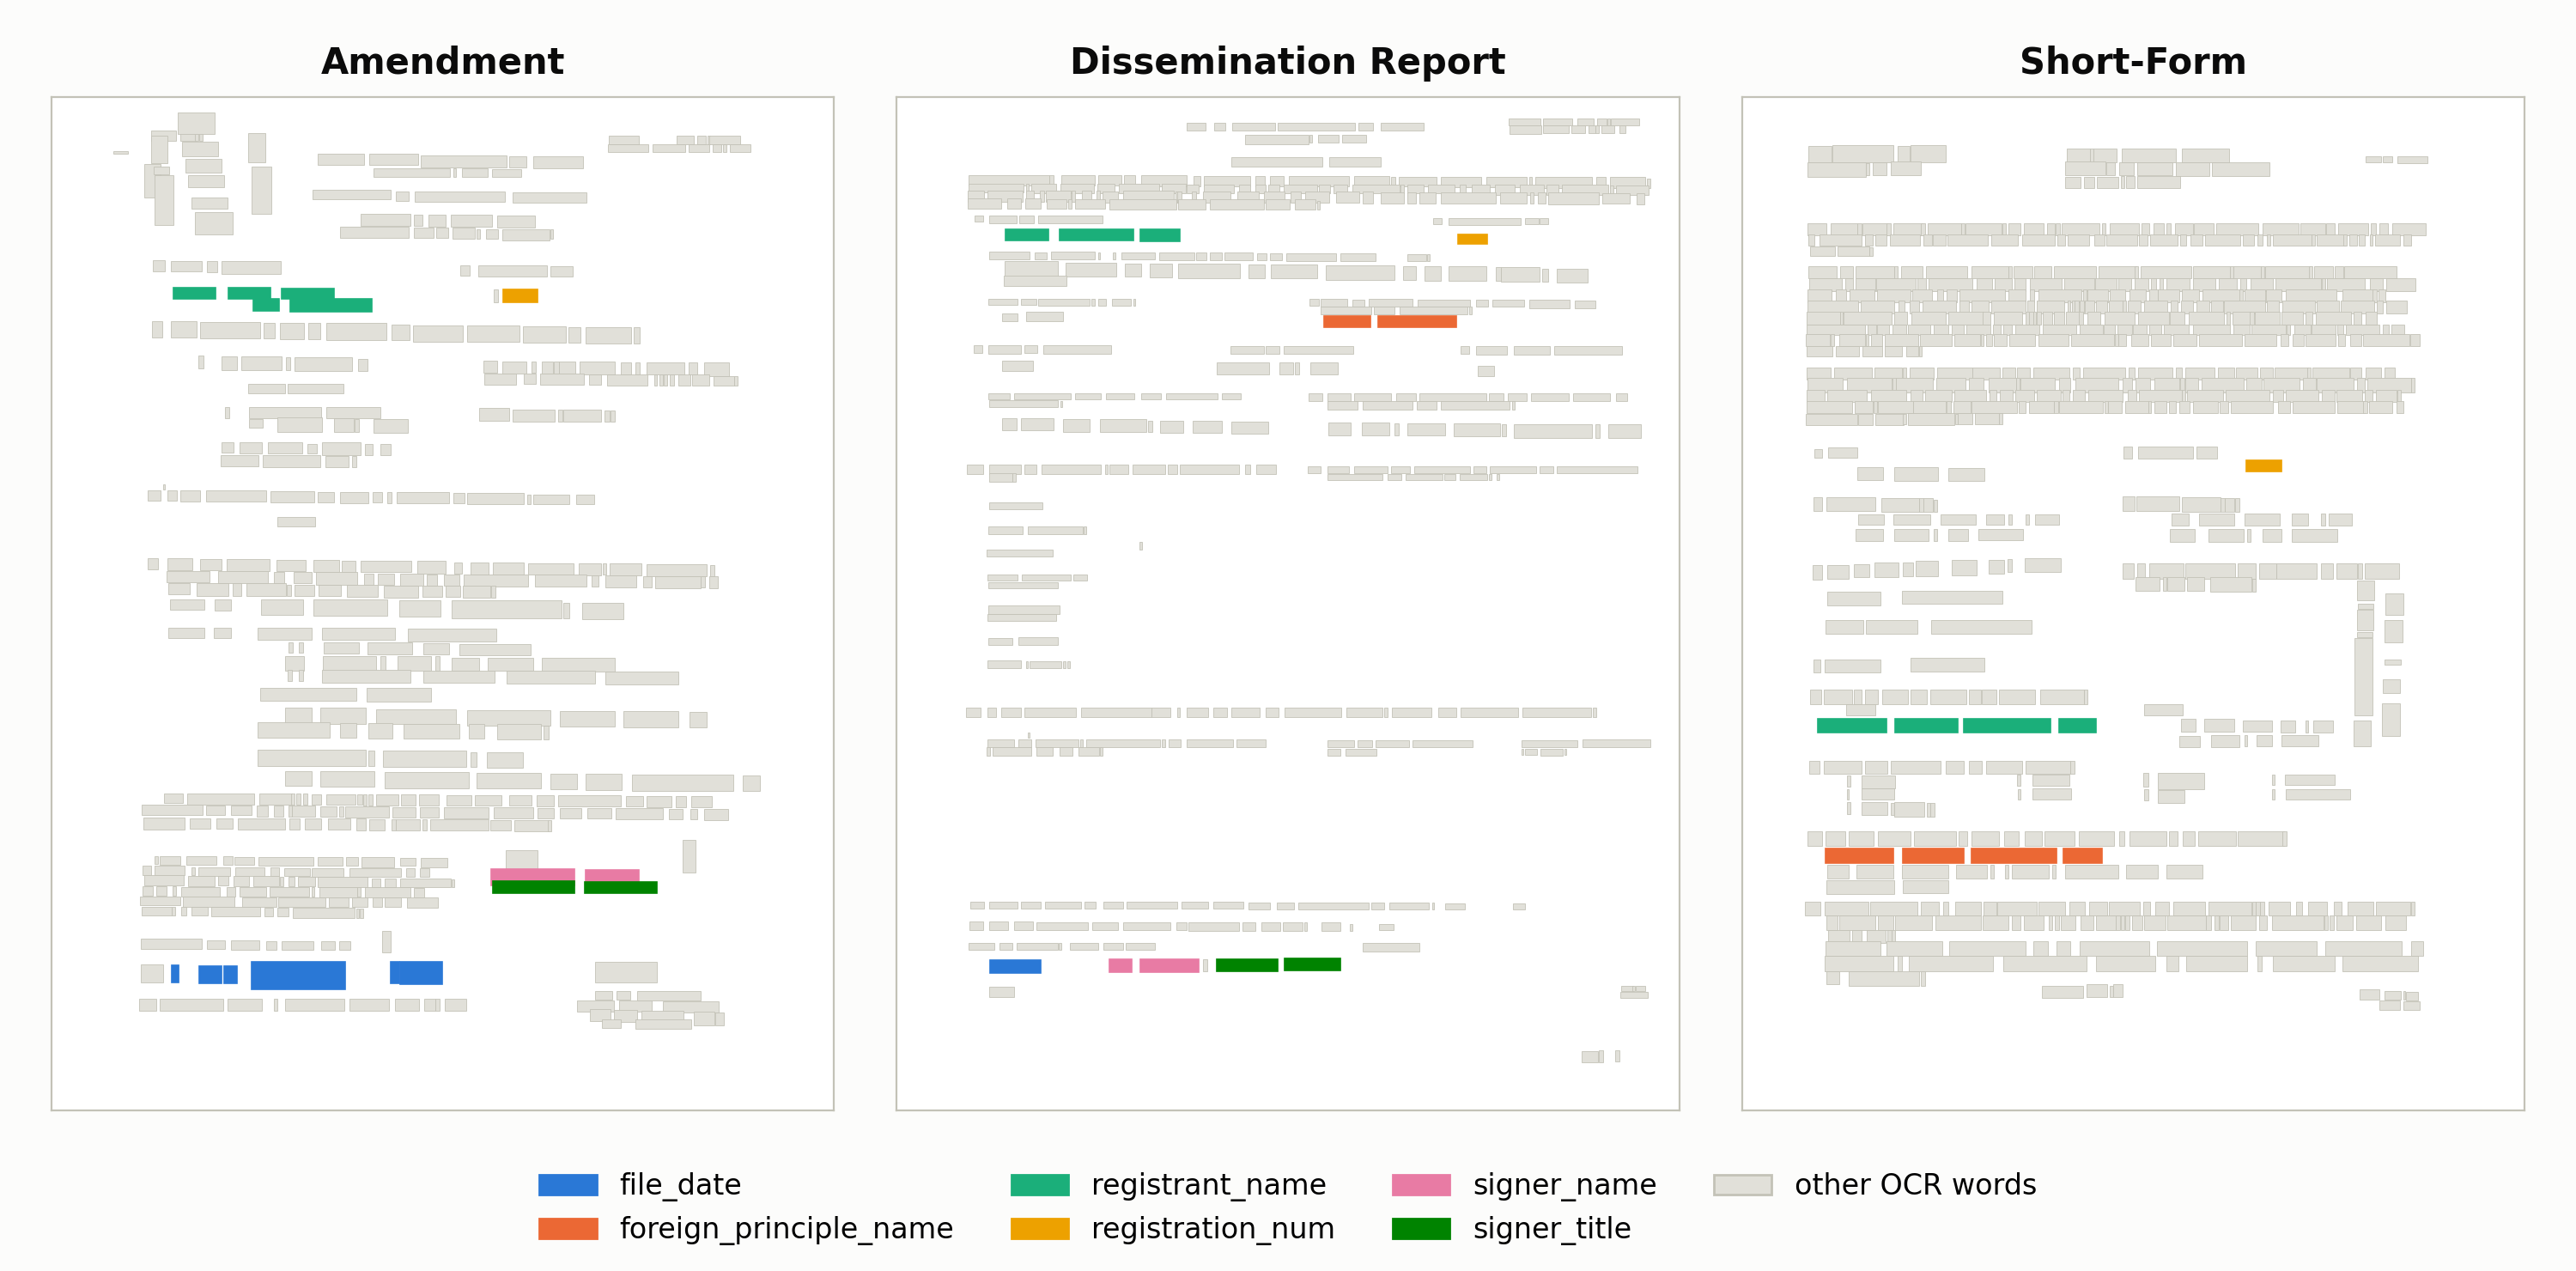
\includegraphics[width=\linewidth]{fig8_template_examples.png}
\caption{Page 1 of one real registration form per template, drawn from VRDU's OCR boxes. Grey boxes are OCR words; coloured boxes are the six labelled fields.}
\label{fig:templates}
\end{figure}

\paragraph{VRDU Ad-Buy forms.} 641 political advertising invoices (the DeepForm data) with nine fields such as advertiser, agency, contract number, flight dates and gross amount, averaging 1,524 words per document. VRDU provides official mixed-template and unseen-template splits for this corpus, and we use them directly.

\paragraph{FUNSD and XFUND.} FUNSD \cite{funsd} has 199 noisy scanned forms with words grouped into entities labelled header, question, answer or other, plus links between related entities (4,147 links in the training set). We use the original release \cite{funsdsite} because the common Hugging Face copy drops the links. XFUND \cite{xfund,xfundrepo} has the same annotation scheme for forms in seven languages; we use Spanish, French, German, Italian and Portuguese. These two datasets are where we train and evaluate linking, because VRDU has no key-value link labels.

\paragraph{Synthetic forms.} To stress-test the pipeline we wrote a generator that draws forms from seven families (invoice, itemised financial statement, procurement order with wrapped tables, shipping manifest, medical intake, ad-buy contract and FARA registration) using PIL with fake values from the Faker library, and degrades some of them with Augraphy \cite{augraphy} to look like scans. Output is in FUNSD format, with entity and link labels (Figure~\ref{fig:synthetic}).

\begin{figure}[H]
\centering
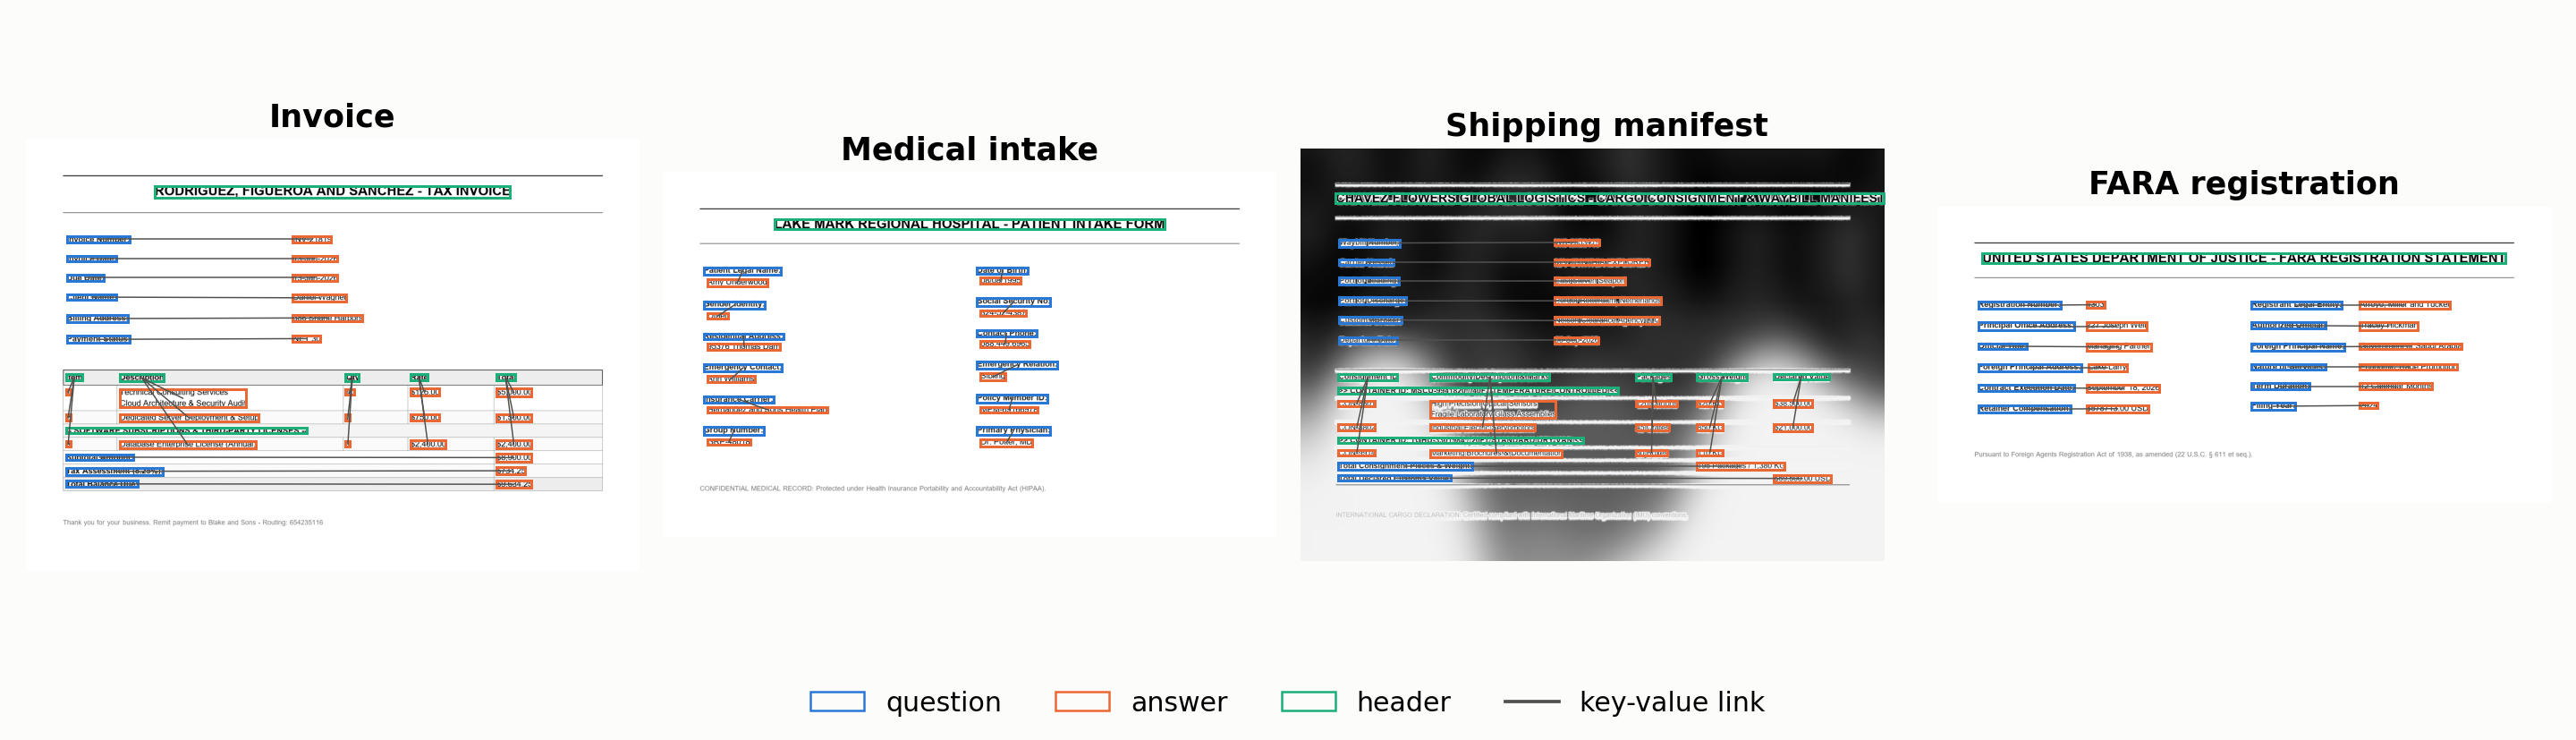
\includegraphics[width=\linewidth]{fig9_synthetic_examples.png}
\caption{Four of the seven synthetic form families with their question, answer and header boxes and key-value links.}
\label{fig:synthetic}
\end{figure}

\paragraph{Preprocessing.}
\begin{itemize}
  \item Word boxes are scaled to integers in $[0,1000]$ relative to the page. Boxes with swapped corners are repaired.
  \item VRDU annotations are aligned to OCR tokens by overlapping character offsets, which is more reliable than matching strings.
  \item Words get BIO tags (13 tags for the registration corpus). During training only the first sub-word of each word carries a label; the rest are ignored in the loss.
  \item For long documents we cut the word sequence into windows of 384 words with an overlap of 128 (Section~\ref{sec:after}).
  \item For the graph models we run the pretrained LiLT once over each window, keep the 768-D vector of each word, build the Delaunay graph and save everything to a feature cache.
\end{itemize}

\paragraph{Splits.} For the unseen-template setting (UTL), each fold holds out one template completely as the test set; 15\% of the remaining documents form the validation set and training is capped at $N=200$. For the seen-template setting (MTL) we stratify by template, keep 20\% for test and 15\% for validation and again cap training at 200. We run 3 folds with 3 seeds (13, 21, 42), so each setting has 9 runs. As an example, the MTL split has 200/286/381 train/validation/test documents, and the UTL fold that holds out Amendment has 200/180/709. VRDU's own unseen-template validation files contain documents from the target template, so we use a stricter version that removes them. Every split goes through \texttt{assert\_no\_template\_leakage}, which fails if a test template appears in training or validation.

% ----------------------------------------------------------------------------
\section{Methods and Approaches}

\subsection{Work done before the prep-presentation review}
\label{sec:before}

\paragraph{Evaluation protocol.} Before training anything we wanted an evaluation we could trust, because a split that leaks templates would make every later number meaningless. We wrote the split code above, the leakage assertion, and two independent implementations of entity F1: \texttt{seqeval} in strict IOB2 mode and our own span matcher. Every run checks that the two agree. We also log how many words were cut off by the 512-token limit and how often the model predicts an \texttt{I-} tag without a matching \texttt{B-}.

\paragraph{LiLT baseline.} Our first model is LiLT with a linear token-classification head. Words and boxes go through the tokenizer, the text stream (a RoBERTa-base encoder) and the layout stream produce 768-D vectors that share attention, and the head predicts a BIO tag per token. The loss is token-level cross-entropy. We used the public \texttt{SCUT-DLVCLab/lilt-roberta-en-base} checkpoint \cite{liltckpt}. LiLT suits the problem because it already knows how to use 2-D position, and its separate layout stream should in principle make it less tied to a particular language or font.

\paragraph{Failure taxonomy.} To analyse errors on unseen templates we sort each wrong prediction into one of four buckets: OCR or recognition error (the text itself is wrong), layout association (right text, attached to the wrong key), field type (right place, wrong label) and repeated structure (line items split or merged).

\paragraph{Results at the review.} LiLT reached 79.29 $\pm$ 1.36 F1 on FUNSD over three seeds, below the published number; we flagged this openly. On VRDU registration forms we measured 87.74 F1 on seen templates and 66.66 on unseen ones, and the taxonomy put 97.2\% of unseen-template errors in the field-type bucket (Figure~\ref{fig:prep}).

\begin{figure}[H]
\centering
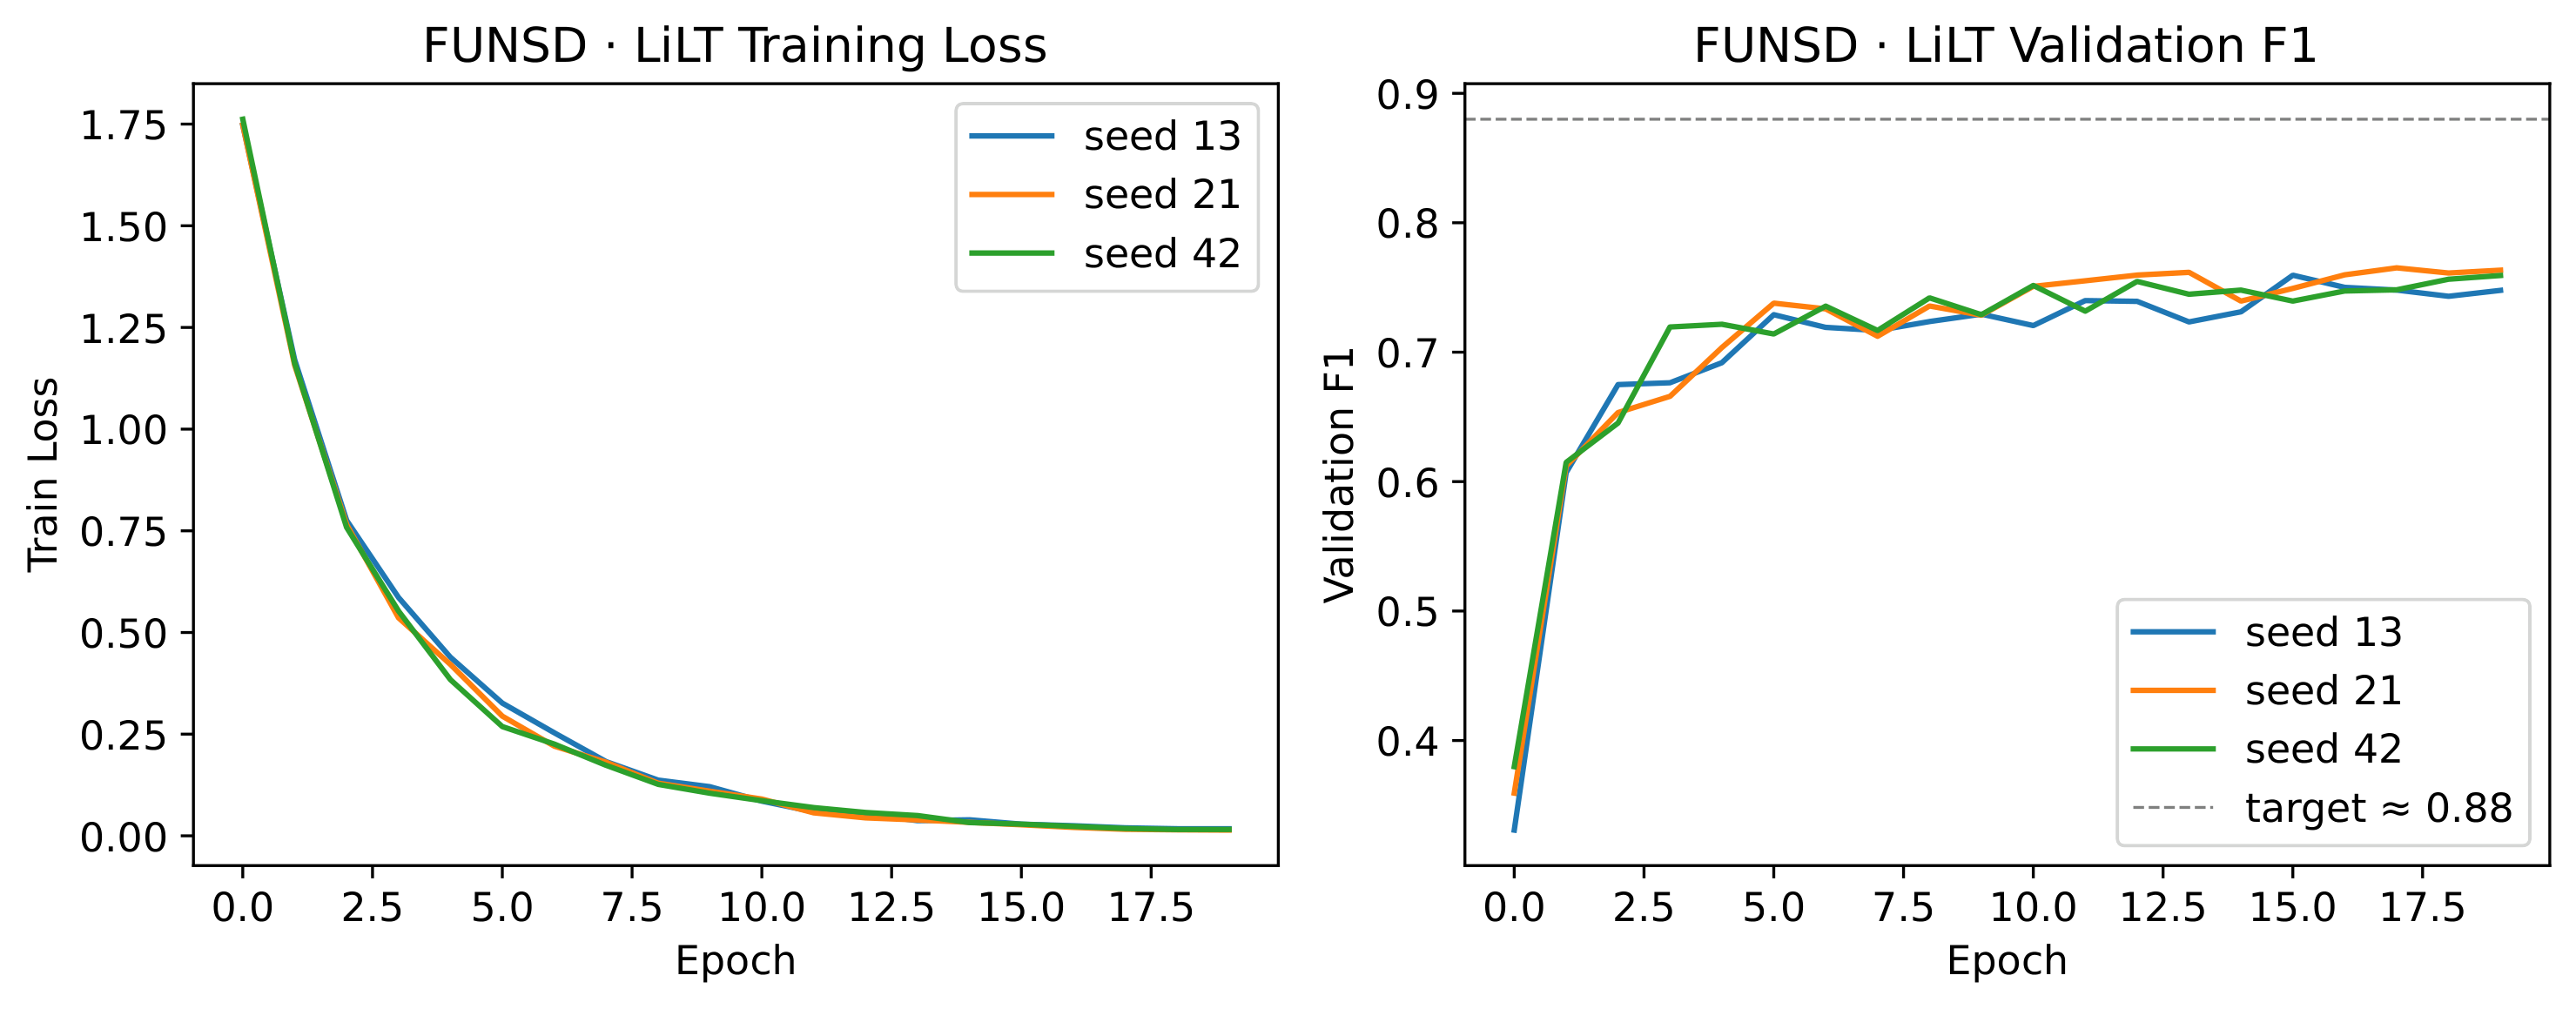
\includegraphics[width=0.56\linewidth]{funsd_curve.png}\hfill
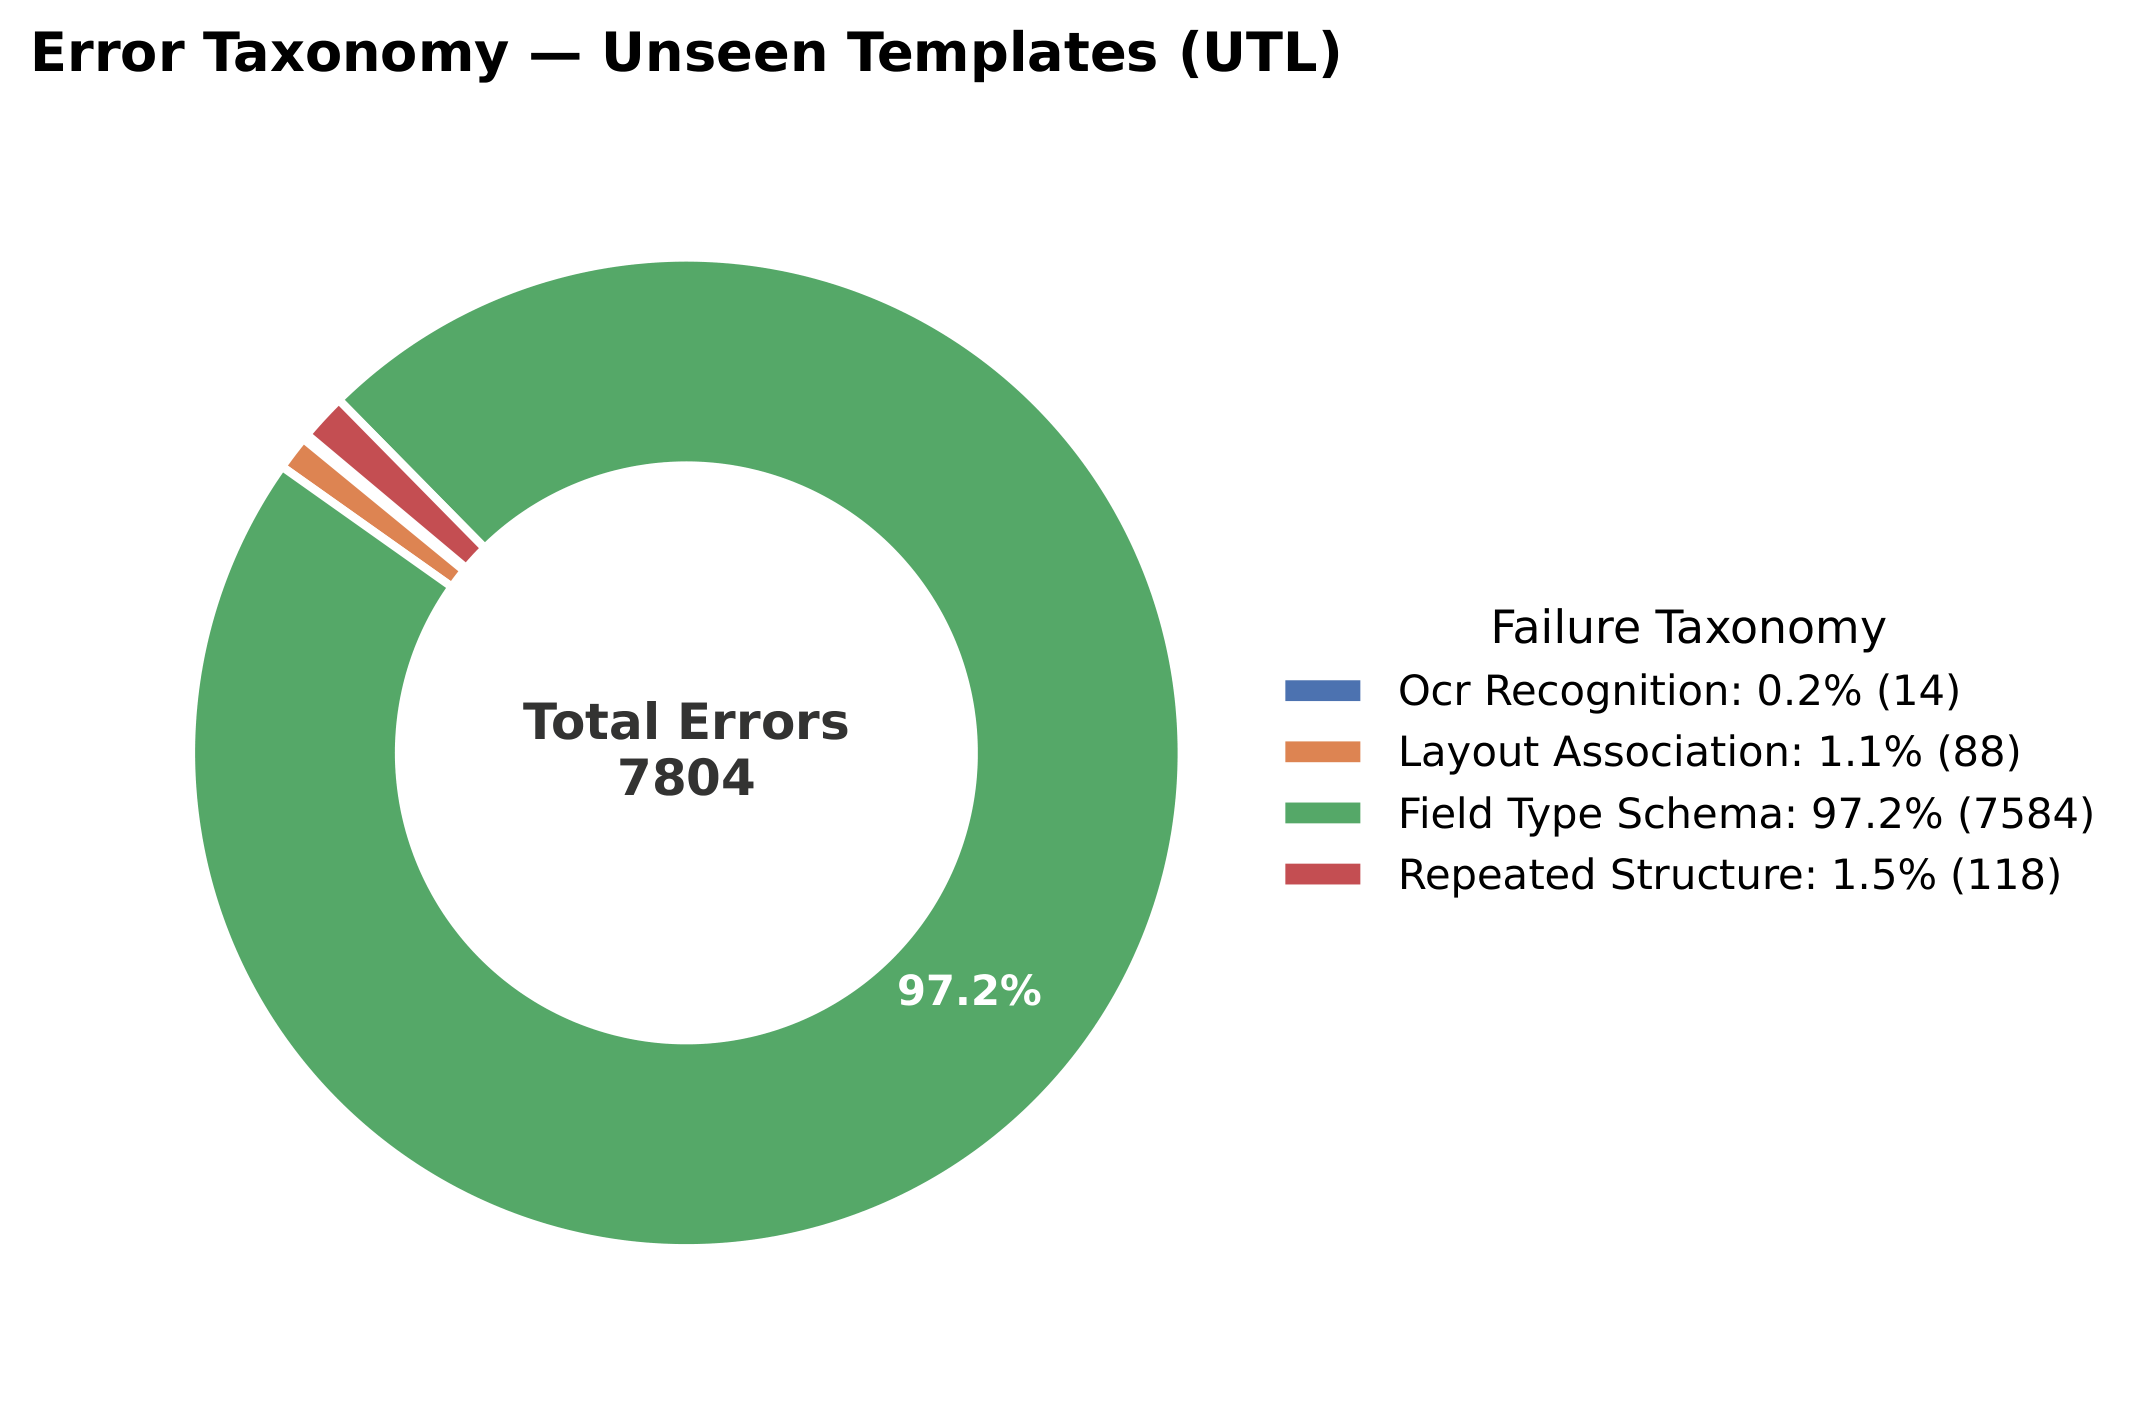
\includegraphics[width=0.40\linewidth]{error_taxonomy.png}
\caption{Left: LiLT training loss and validation F1 on FUNSD for three seeds. Right: pilot error taxonomy on unseen VRDU templates (7,804 errors).}
\label{fig:prep}
\end{figure}

\subsection{Work done after the prep-presentation review}
\label{sec:after}

\paragraph{Sliding windows and coordinate anchoring.} The prep-review logs showed that on long registration documents most words never reached the model because of the 512-token limit. We now cut each document into windows of 384 words that overlap by 128. At test time each window is classified on its own, the softmax probabilities of a word are summed over all windows that contain it, and the word gets the argmax. We also added two training-time changes aimed at position memorisation: random coordinate jitter (shift up to $\pm$80 units, scale 0.85 to 1.15) and re-anchoring the boxes relative to the bounding box of the page's content.

\paragraph{Joint tagging and key-value linking.} The task asks for key-value pairs, and a tagger alone only labels words. We added a relation head on top of LiLT. Each entity is represented by the mean of its first-sub-word vectors, and two small MLPs ($768 \to 128$, LayerNorm, GELU, dropout 0.1) map it to a "head" vector $h_i$ and a "tail" vector $t_j$. The score for linking entity $i$ (key) to entity $j$ (value) is biaffine \cite{biaffine}:
\begin{equation}
s(i \to j) = h_i^\top W t_j + w^\top [\,h_i;\, t_j;\, \phi(b_i, b_j)\,] + c,
\end{equation}
where $\phi(b_i,b_j)$ is a 64-D embedding of 16 hand-designed spatial features of the two boxes:
\begin{itemize}
  \item geometry (5): horizontal and vertical centre offsets, distance, and the cosine and sine of the angle between centres;
  \item containment (5): overlap in $x$ and in $y$ relative to the smaller box, whether the boxes are disjoint in $x$ and in $y$, and whether $j$ lies below $i$;
  \item line of sight (2): whether any other box blocks the horizontal or the vertical ray between them;
  \item typography (4): log ratios of box heights and areas, and the z-scored heights of both boxes.
\end{itemize}
A soft type prior subtracts 5 from the score of type pairs that should not link (anything other than question$\to$answer, header$\to$question and header$\to$answer). The joint loss is $L = L_{\text{tag}} + \lambda L_{\text{link}}$ with $\lambda = 1$. Because only a few percent of all entity pairs are real links, we use focal loss \cite{focal} for $L_{\text{link}}$, with $\gamma = 2$ and $\alpha = 0.75$, normalised by the number of positive links. At decoding time each value keeps only its highest-scoring key, and only if the probability is at least 0.5 ("one-to-one" decoding).

Training the encoder and the link head together from the start was unstable, so we use a three-phase curriculum. Phase 1 trains tagging only and keeps the checkpoint with the best validation entity F1. Phase 2 freezes the encoder and trains the link head on gold entity spans, selecting on validation linking F1. Phase 3 trains everything jointly, with the encoder learning rate scaled by 0.2, selecting on the average of the two F1 scores. Each phase starts from the best weights of the previous one.

\paragraph{Delaunay word graph with Edge-GAT (RSA-GNN).} Our hypothesis was that the position of a word relative to its neighbours would carry over to new templates better than its absolute position on the page. Each word becomes a node with its 768-D LiLT vector. Edges come from a Delaunay triangulation of the word centres, made bidirectional; if the page image is available, edges that cross ruled lines found with OpenCV morphology are removed. Each edge carries the same 16 spatial features as above. Our Edge-GAT layer, based on GAT \cite{gat}, puts the edge features inside the attention score:
\begin{equation}
\alpha_{ij} = \operatorname{softmax}_{j \in \mathcal{N}(i)}\!\big(a^\top \mathrm{LeakyReLU}(W_s h_i + W_d h_j + W_e e_{ij})\big),
\qquad
h_i' = \sum_{j} \alpha_{ij}\,(W_v h_j + W_{ve} e_{ij}),
\end{equation}
followed by a residual connection, LayerNorm and GELU. The model projects 768 to 256 dimensions, stacks one to three such layers with 4 heads of 64 dimensions and dropout 0.1, and classifies each node into the 13 BIO tags with a two-layer MLP. The loss is cross-entropy.

\paragraph{NER-fused joint GNN.} This variant appends an 8-D one-hot entity type from regular expressions (date, money, ID, name, location, text, punctuation, other) to each node, giving 776-D inputs, and has two heads: a node head that predicts key, value, header or other, and an edge head, an MLP on $[h_i \,\|\, h_j \,\|\, e_{ij}]$, that predicts whether an edge is a key-value link. The loss is node cross-entropy plus $1.5\times$ focal loss on edges. Since VRDU has no link labels, the node roles and edge links are derived heuristically: a value is any labelled entity token, a key is a word ending in a colon or a word just before an entity, and a link connects a key to a value that does not start to its left.

% ----------------------------------------------------------------------------
\section{Experiments}

\begin{table}[H]
\centering\small
\caption{Training settings.}
\label{tab:setup}
\begin{tabular}{@{}lll@{}}
\toprule
Setting & LiLT models & Graph models \\
\midrule
Optimizer & AdamW, learning rate $5\times10^{-5}$, weight decay 0.01 & AdamW, $10^{-3}$, weight decay $10^{-4}$ \\
Learning-rate schedule & OneCycle, 10\% warm-up, linear annealing & constant \\
Epochs & 20; XFUND curriculum capped at 8 / 6 / 8 & 20 (matched runs), 30 (ablations) \\
Batch size & 4 documents & 4 (matched), 16 (ablations) \\
Early stopping & patience 3 epochs, minimum gain 0.001 & best validation checkpoint \\
Gradient clipping & norm 1.0 & norm 1.0 (ablations) \\
Seeds & 13, 21, 42 & 13, 42 \\
\bottomrule
\end{tabular}
\end{table}

\paragraph{Experiments run.}
\begin{enumerate}
  \item LiLT on FUNSD, 3 seeds (pipeline check).
  \item LiLT on VRDU registration forms, MTL vs UTL, 3 folds $\times$ 3 seeds per setting, $N=200$.
  \item The same on VRDU Ad-Buy forms with the official splits.
  \item LiLT with sliding windows and coordinate anchoring on both corpora.
  \item Joint LiLT tagging and linking on FUNSD (first version, 10 spatial features, no curriculum) and on XFUND (curriculum, focal loss, one-to-one decoding).
  \item Seven-condition ablation on XFUND: full 16-D model; without line of sight; without typography; without containment; geometry only; BCE instead of focal loss; independent decoding instead of one-to-one.
  \item Edge-GAT ablations on registration forms with a random 80/10/10 document split: plain GAT without edge features, 16-D edges with 2 layers, 1 layer, 3 layers.
  \item RSA-GNN and NER-fused GNN under the matched MTL/UTL protocol.
  \item Joint LiLT on the synthetic forms.
\end{enumerate}

\paragraph{Metrics.} Entity F1 is strict IOB2 span F1, micro-averaged over fields, computed with \texttt{seqeval} and checked against our own implementation. Linking F1 counts a predicted key-value pair as correct only if both entity indices match the gold pair. For the NER-fused GNN we report edge-level link F1 over Delaunay edges. The generalisation gap is the mean MTL F1 minus the mean UTL F1, with the relative drop as a percentage of MTL F1.

\paragraph{Hardware.} All training ran on Kaggle notebooks with two NVIDIA Tesla T4 GPUs (16 GB each). Different seeds and folds run as separate processes, one per GPU; we do not split a single model across GPUs. Training is in FP32. Code, configurations and result files are at \url{https://github.com/ABasakEE/KeyValue-Extraction} \cite{ourrepo}.

% ----------------------------------------------------------------------------
\section{Results}

\subsection{Seen versus unseen templates}

\begin{table}[H]
\centering\small
\caption{LiLT entity F1 (\%) under the matched protocol ($N=200$, 9 runs per setting). Mean $\pm$ standard deviation.}
\label{tab:gap}
\begin{tabular}{@{}lccc@{}}
\toprule
Corpus & Seen (MTL) & Unseen (UTL) & Gap (relative) \\
\midrule
VRDU Registration & 87.74 $\pm$ 1.62 & 66.66 $\pm$ 7.29 & 21.08 (24.0\%) \\
\quad held out: Amendment & & 65.82 $\pm$ 1.24 & \\
\quad held out: Dissemination Report & & 74.77 $\pm$ 3.68 & \\
\quad held out: Short-Form & & 59.39 $\pm$ 4.32 & \\
VRDU Ad-Buy & 92.46 $\pm$ 0.86 & 90.61 $\pm$ 1.12 & 1.85 (2.0\%) \\
VRDU Registration, with windows + anchoring & 91.56 & 64.24 & 27.31 (29.8\%) \\
\bottomrule
\end{tabular}
\end{table}

\begin{figure}[H]
\centering
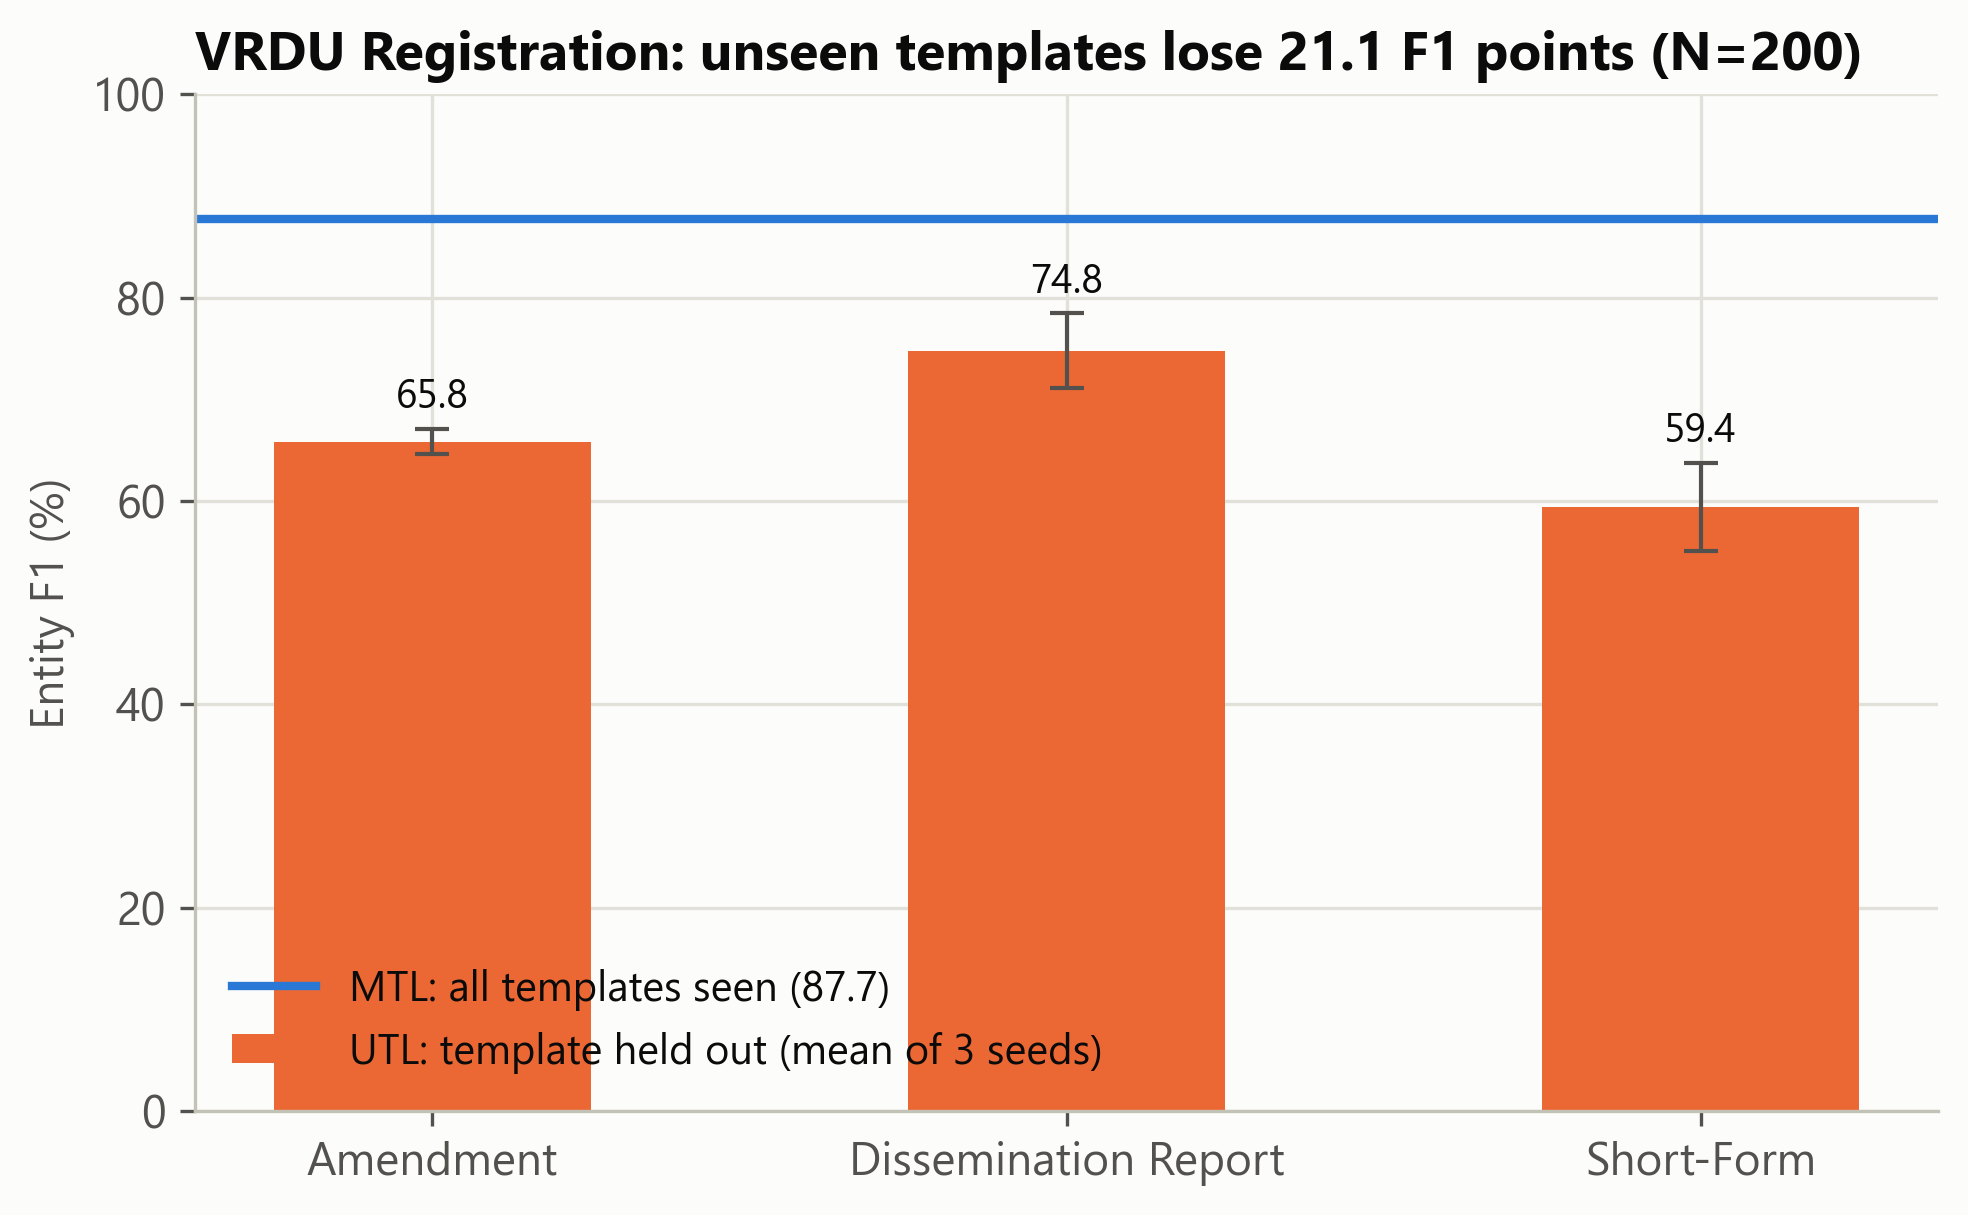
\includegraphics[width=0.49\linewidth]{fig1_gap_per_template.png}\hfill
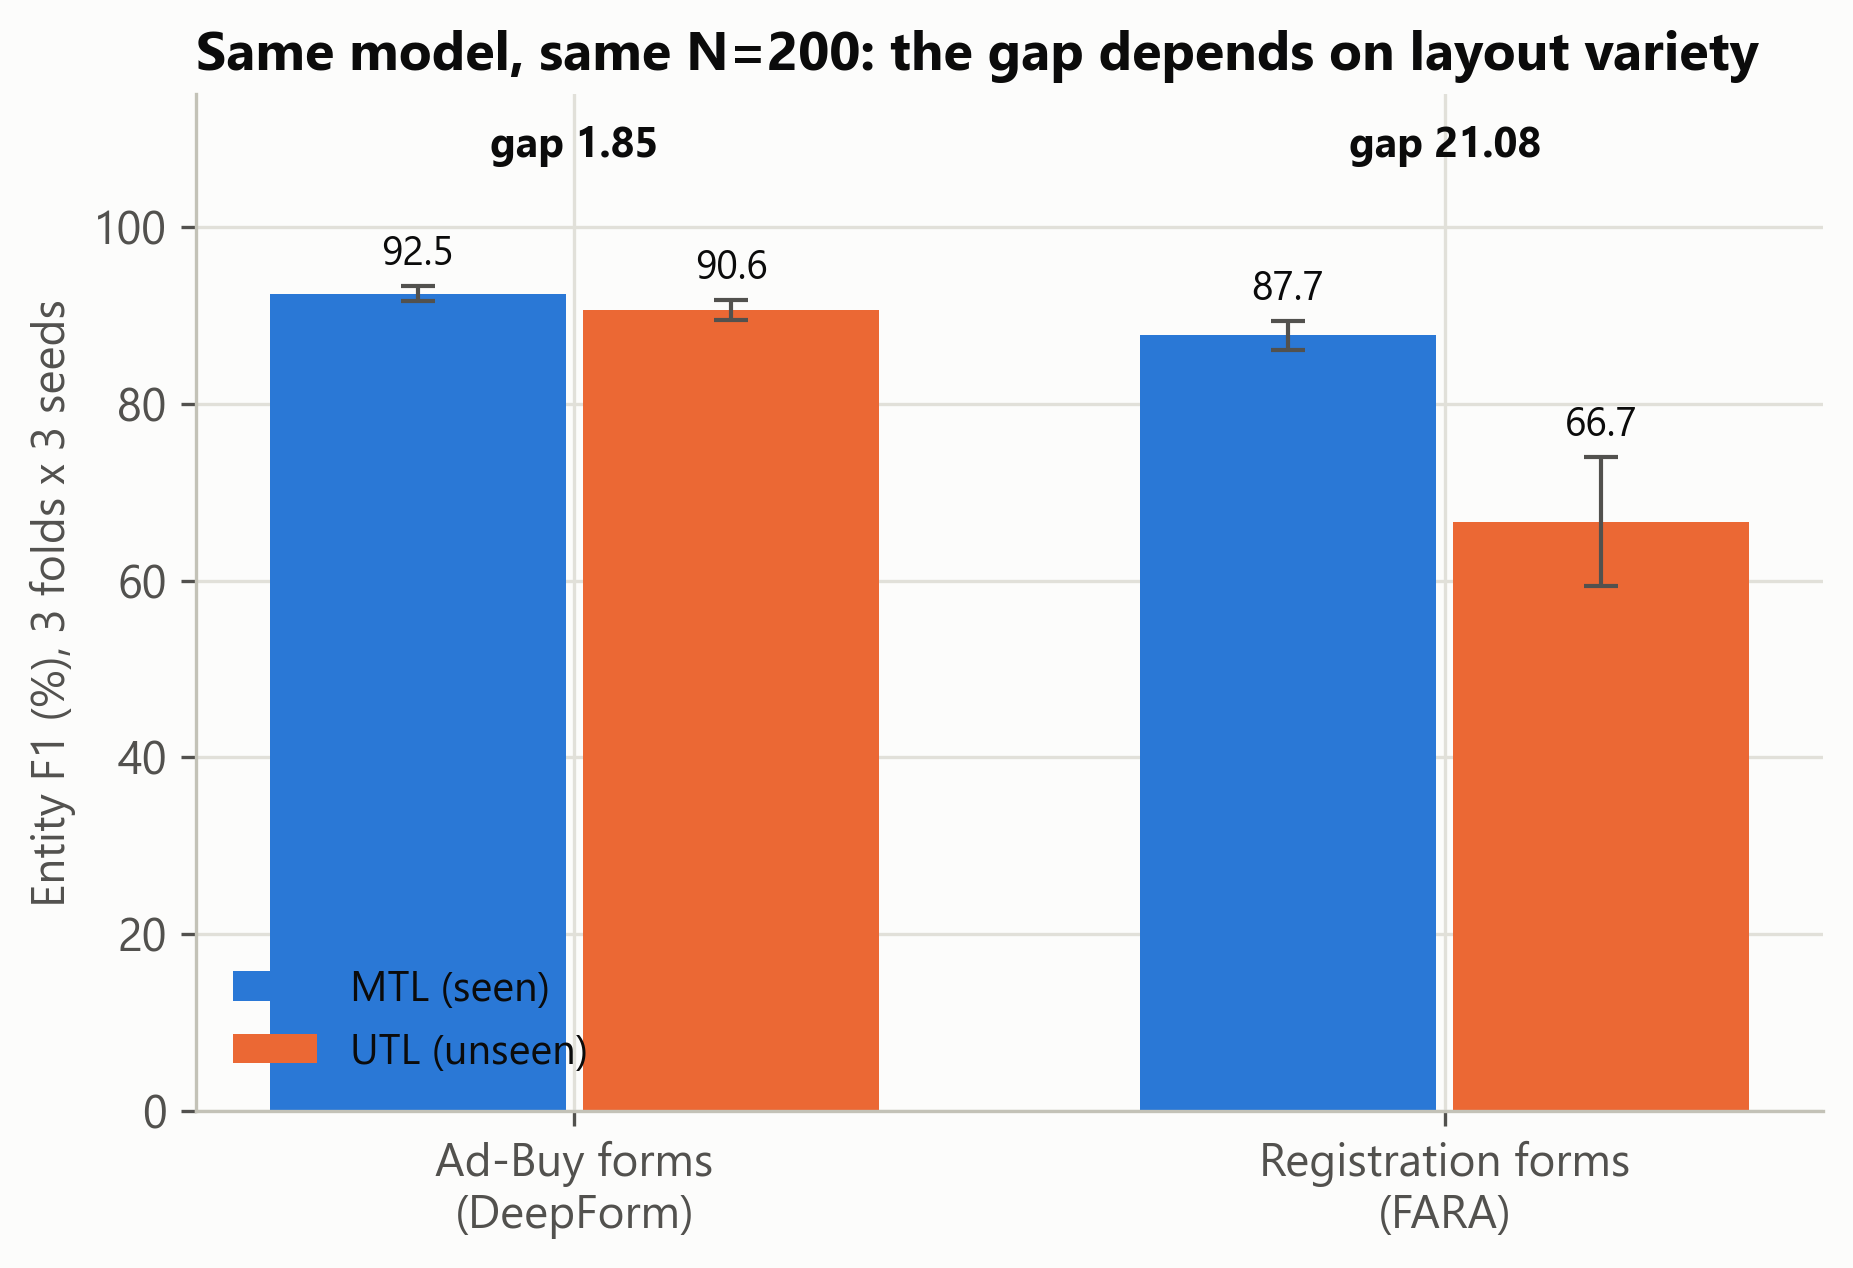
\includegraphics[width=0.49\linewidth]{fig3_adbuy_vs_registration.png}
\caption{Left: unseen-template F1 for each held-out registration template, against the seen-template mean. Right: the same model on Ad-Buy and registration forms.}
\label{fig:gap}
\end{figure}

Table~\ref{tab:gap} and Figure~\ref{fig:gap} show three things. First, the gap on registration forms is large: 21 points, with a standard deviation across runs about four times larger than in the seen setting. Second, the gap depends on the held-out template. Short-Form is the hardest to generalise to and Dissemination Report the easiest. Third, the same model, trained on the same number of documents, loses only 1.85 points on Ad-Buy forms. The Ad-Buy invoices look much more alike than the three registration templates, which are laid out very differently (Figure~\ref{fig:templates}). The size of the gap is therefore a property of how different the templates are, and a single number for "template generalisation" can be misleading without that context.

Sliding windows and anchoring raised seen-template F1 from 87.74 to 91.56 because the model now sees every word, but unseen-template F1 did not improve (64.24), so the gap grew to 27.31. Seeing more of the document helped the model fit the templates it knows without helping it on new ones.

\subsection{Failure analysis}

\begin{figure}[H]
\centering
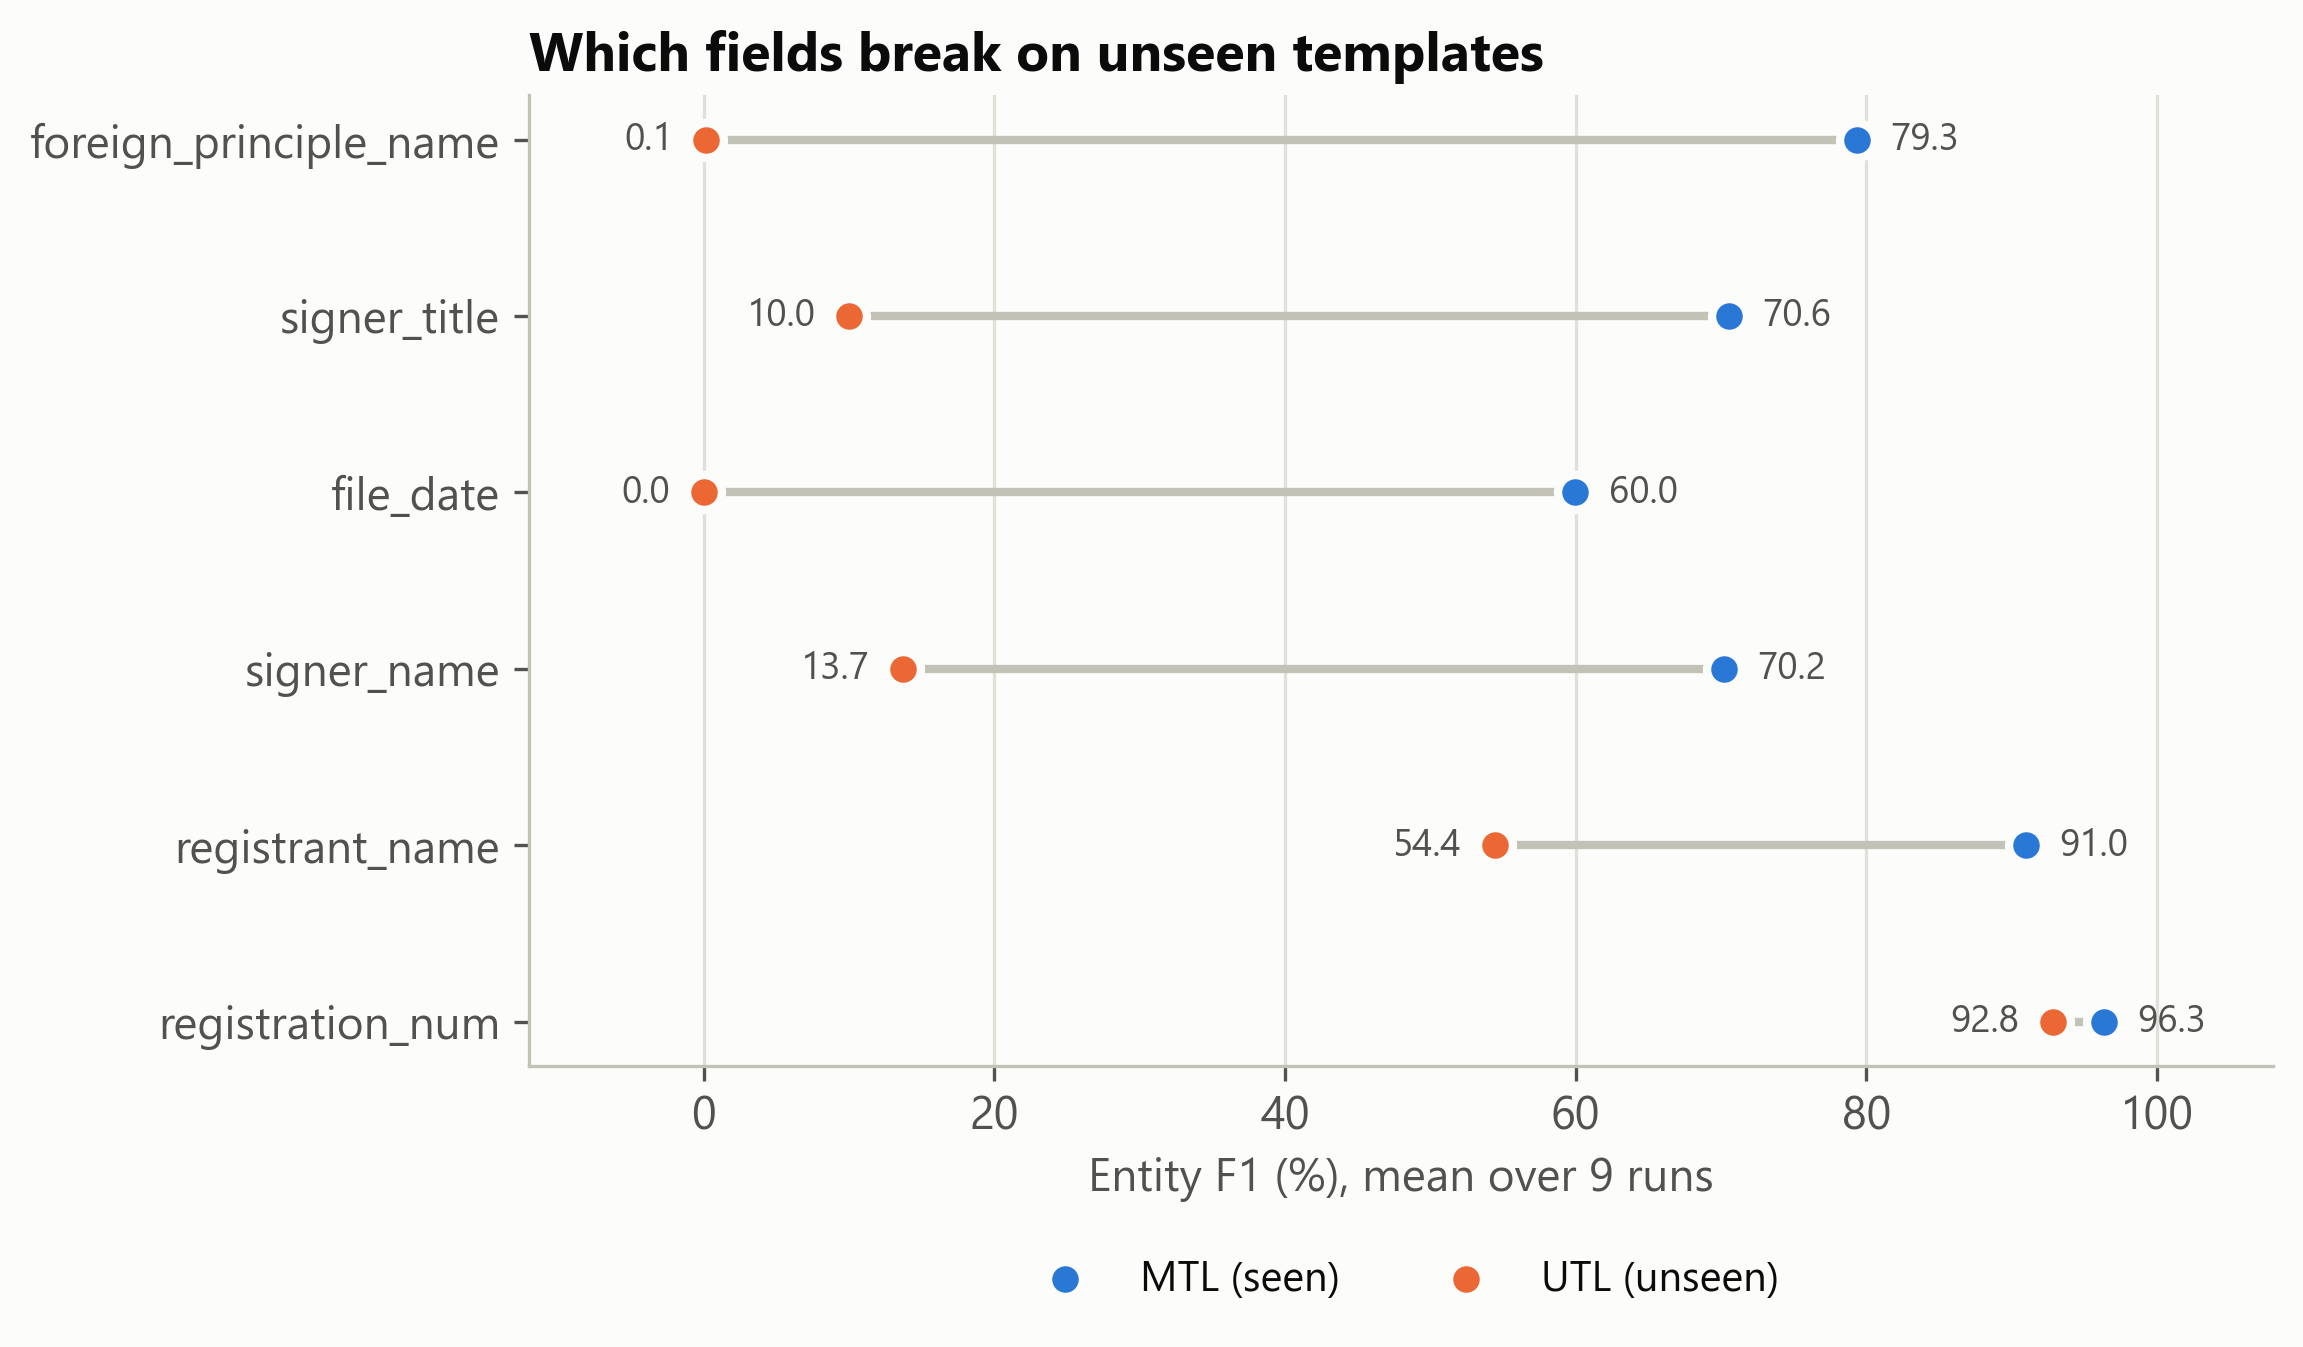
\includegraphics[width=0.62\linewidth]{fig2_per_entity_collapse.png}
\caption{Per-field entity F1 on registration forms, mean over 9 runs per setting.}
\label{fig:entity}
\end{figure}

Figure~\ref{fig:entity} breaks the gap down by field. \texttt{file\_date} drops from 59.98 to 0.00 and \texttt{foreign\_principle\_name} from 79.35 to 0.15. \texttt{signer\_name} and \texttt{signer\_title} fall to 13.72 and 10.00. At the other end, \texttt{registration\_num} keeps 92.83 (from 96.33). Looking at the forms in Figure~\ref{fig:templates} explains the pattern. A date or a person's name looks like many other dates and names on the page, so the model has to rely on where the field usually sits, and that position changes from template to template. A registration number has a distinctive format that reads the same wherever it is printed. This matches the pilot taxonomy, where 97.2\% of unseen-template errors were field-type errors and only 0.2\% came from OCR: the model usually finds text in roughly the right region but cannot tell which field it is.

\begin{figure}[H]
\centering
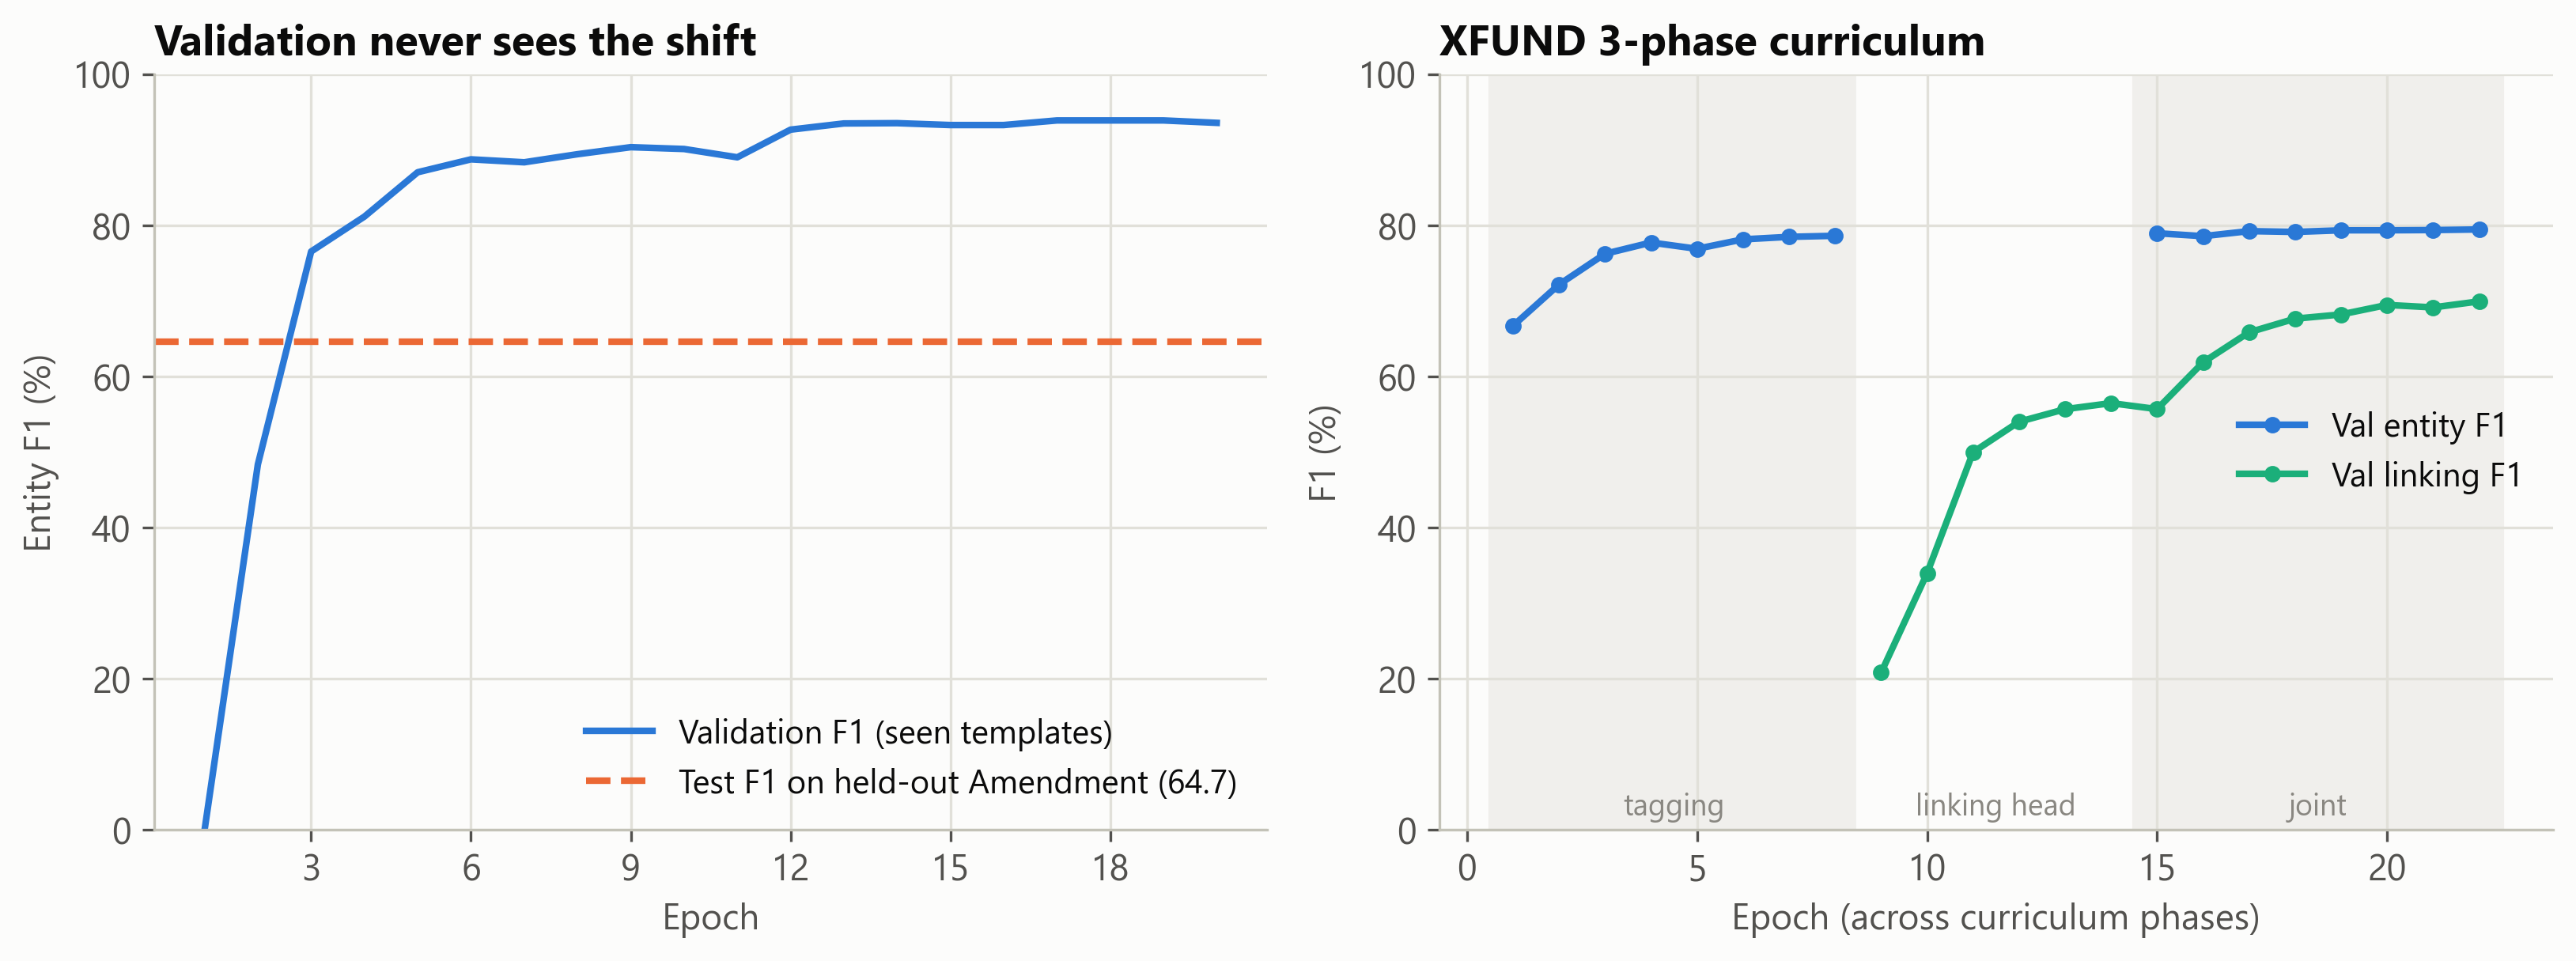
\includegraphics[width=0.9\linewidth]{fig7_training_curves.png}
\caption{Left: validation F1 on seen templates against the final unseen-template test F1 for one UTL run (Amendment held out, seed 42). Right: validation entity and linking F1 through the three curriculum phases on XFUND.}
\label{fig:curves}
\end{figure}

Figure~\ref{fig:curves} (left) shows a practical problem. In the Amendment fold with seed 42, validation F1 reaches 93.9 while the test F1 on the held-out template is 64.7. Validation data from the training templates gives no warning of the drop, so model selection and early stopping cannot catch it. Any real deployment would need some held-out-template validation to notice.

\subsection{Graph models}

\begin{figure}[H]
\centering
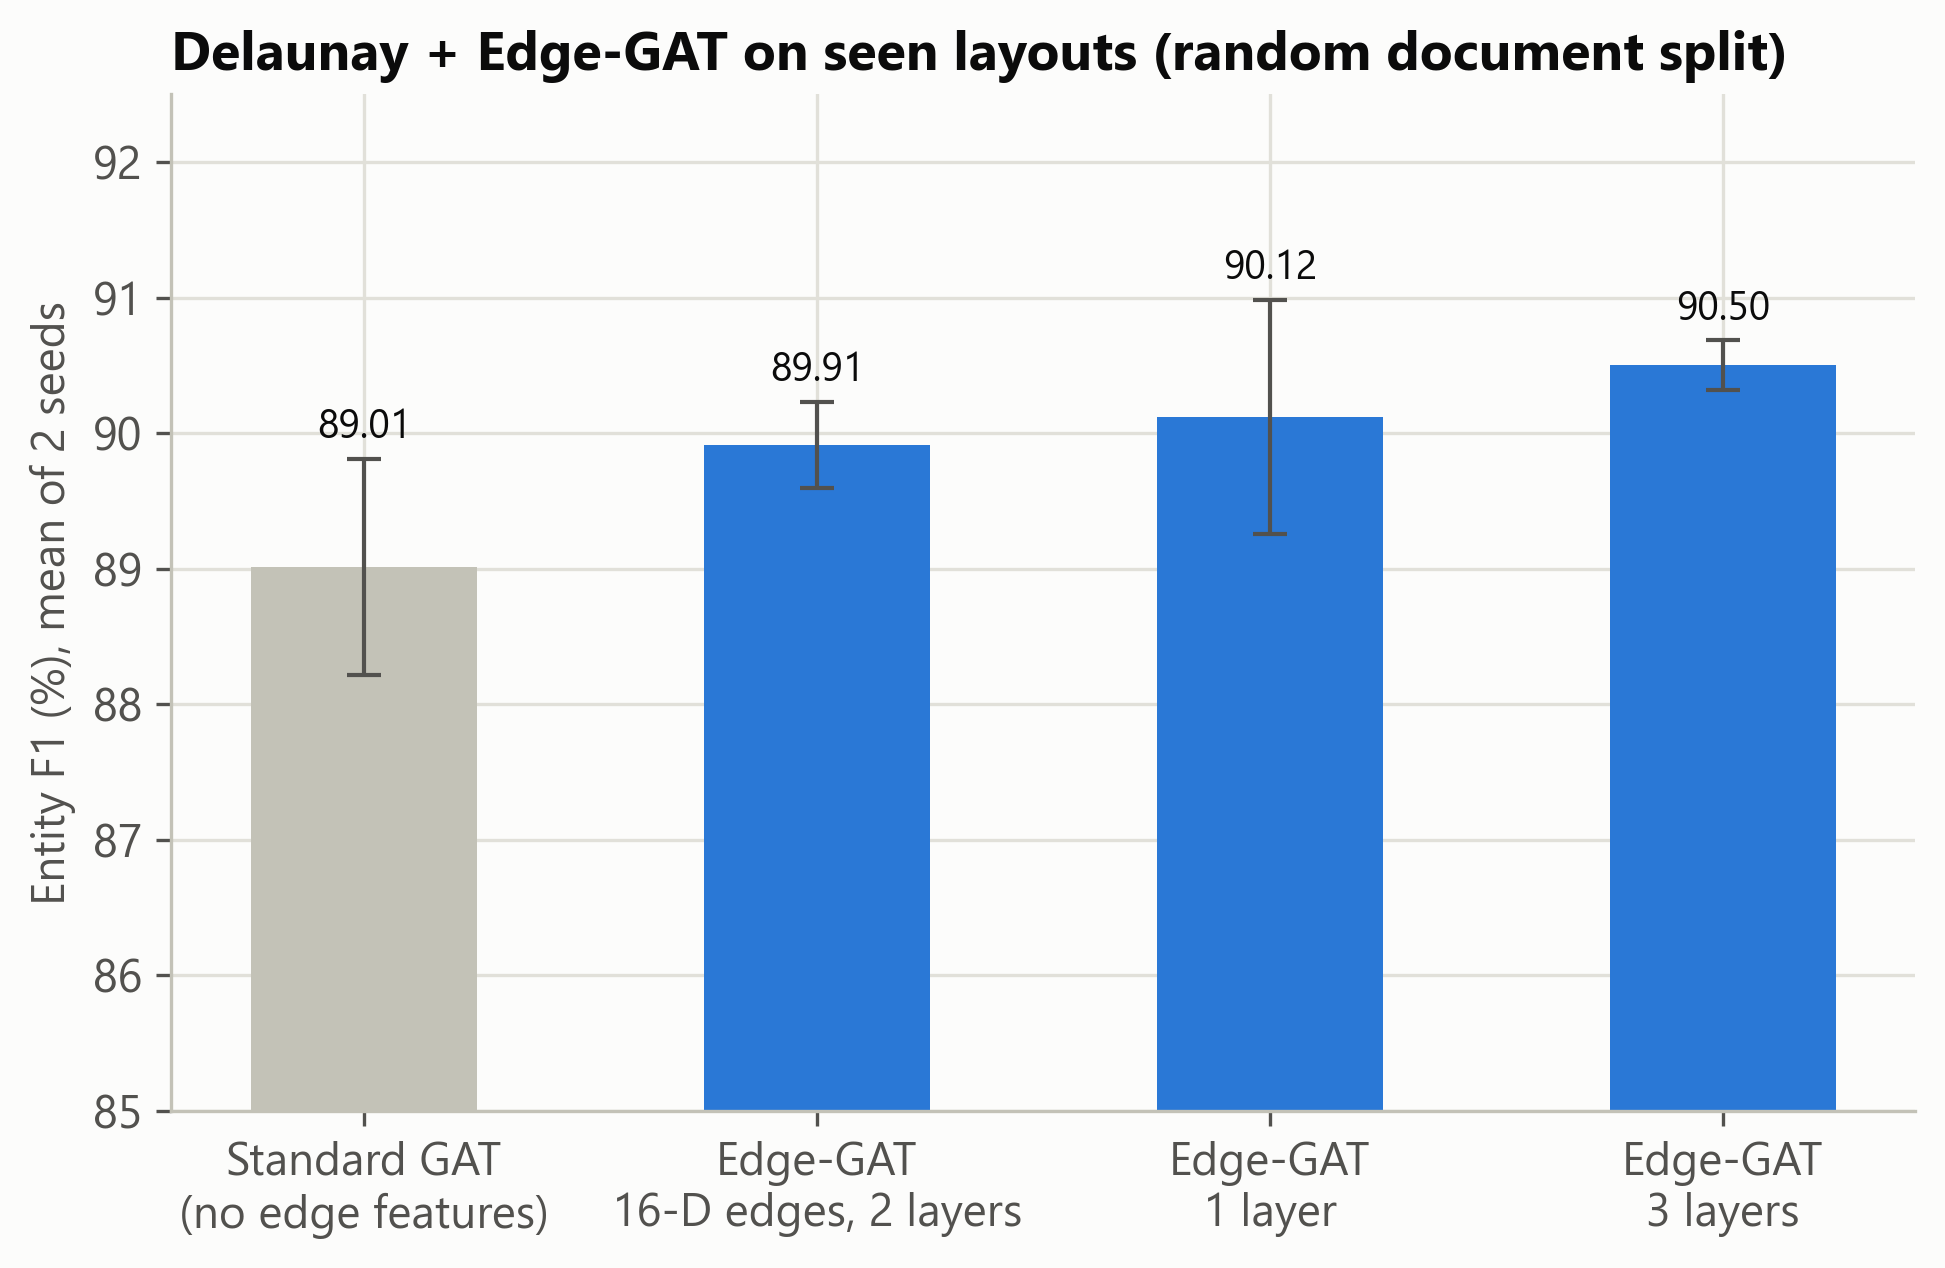
\includegraphics[width=0.40\linewidth]{fig4_gnn_ablations.png}\hfill
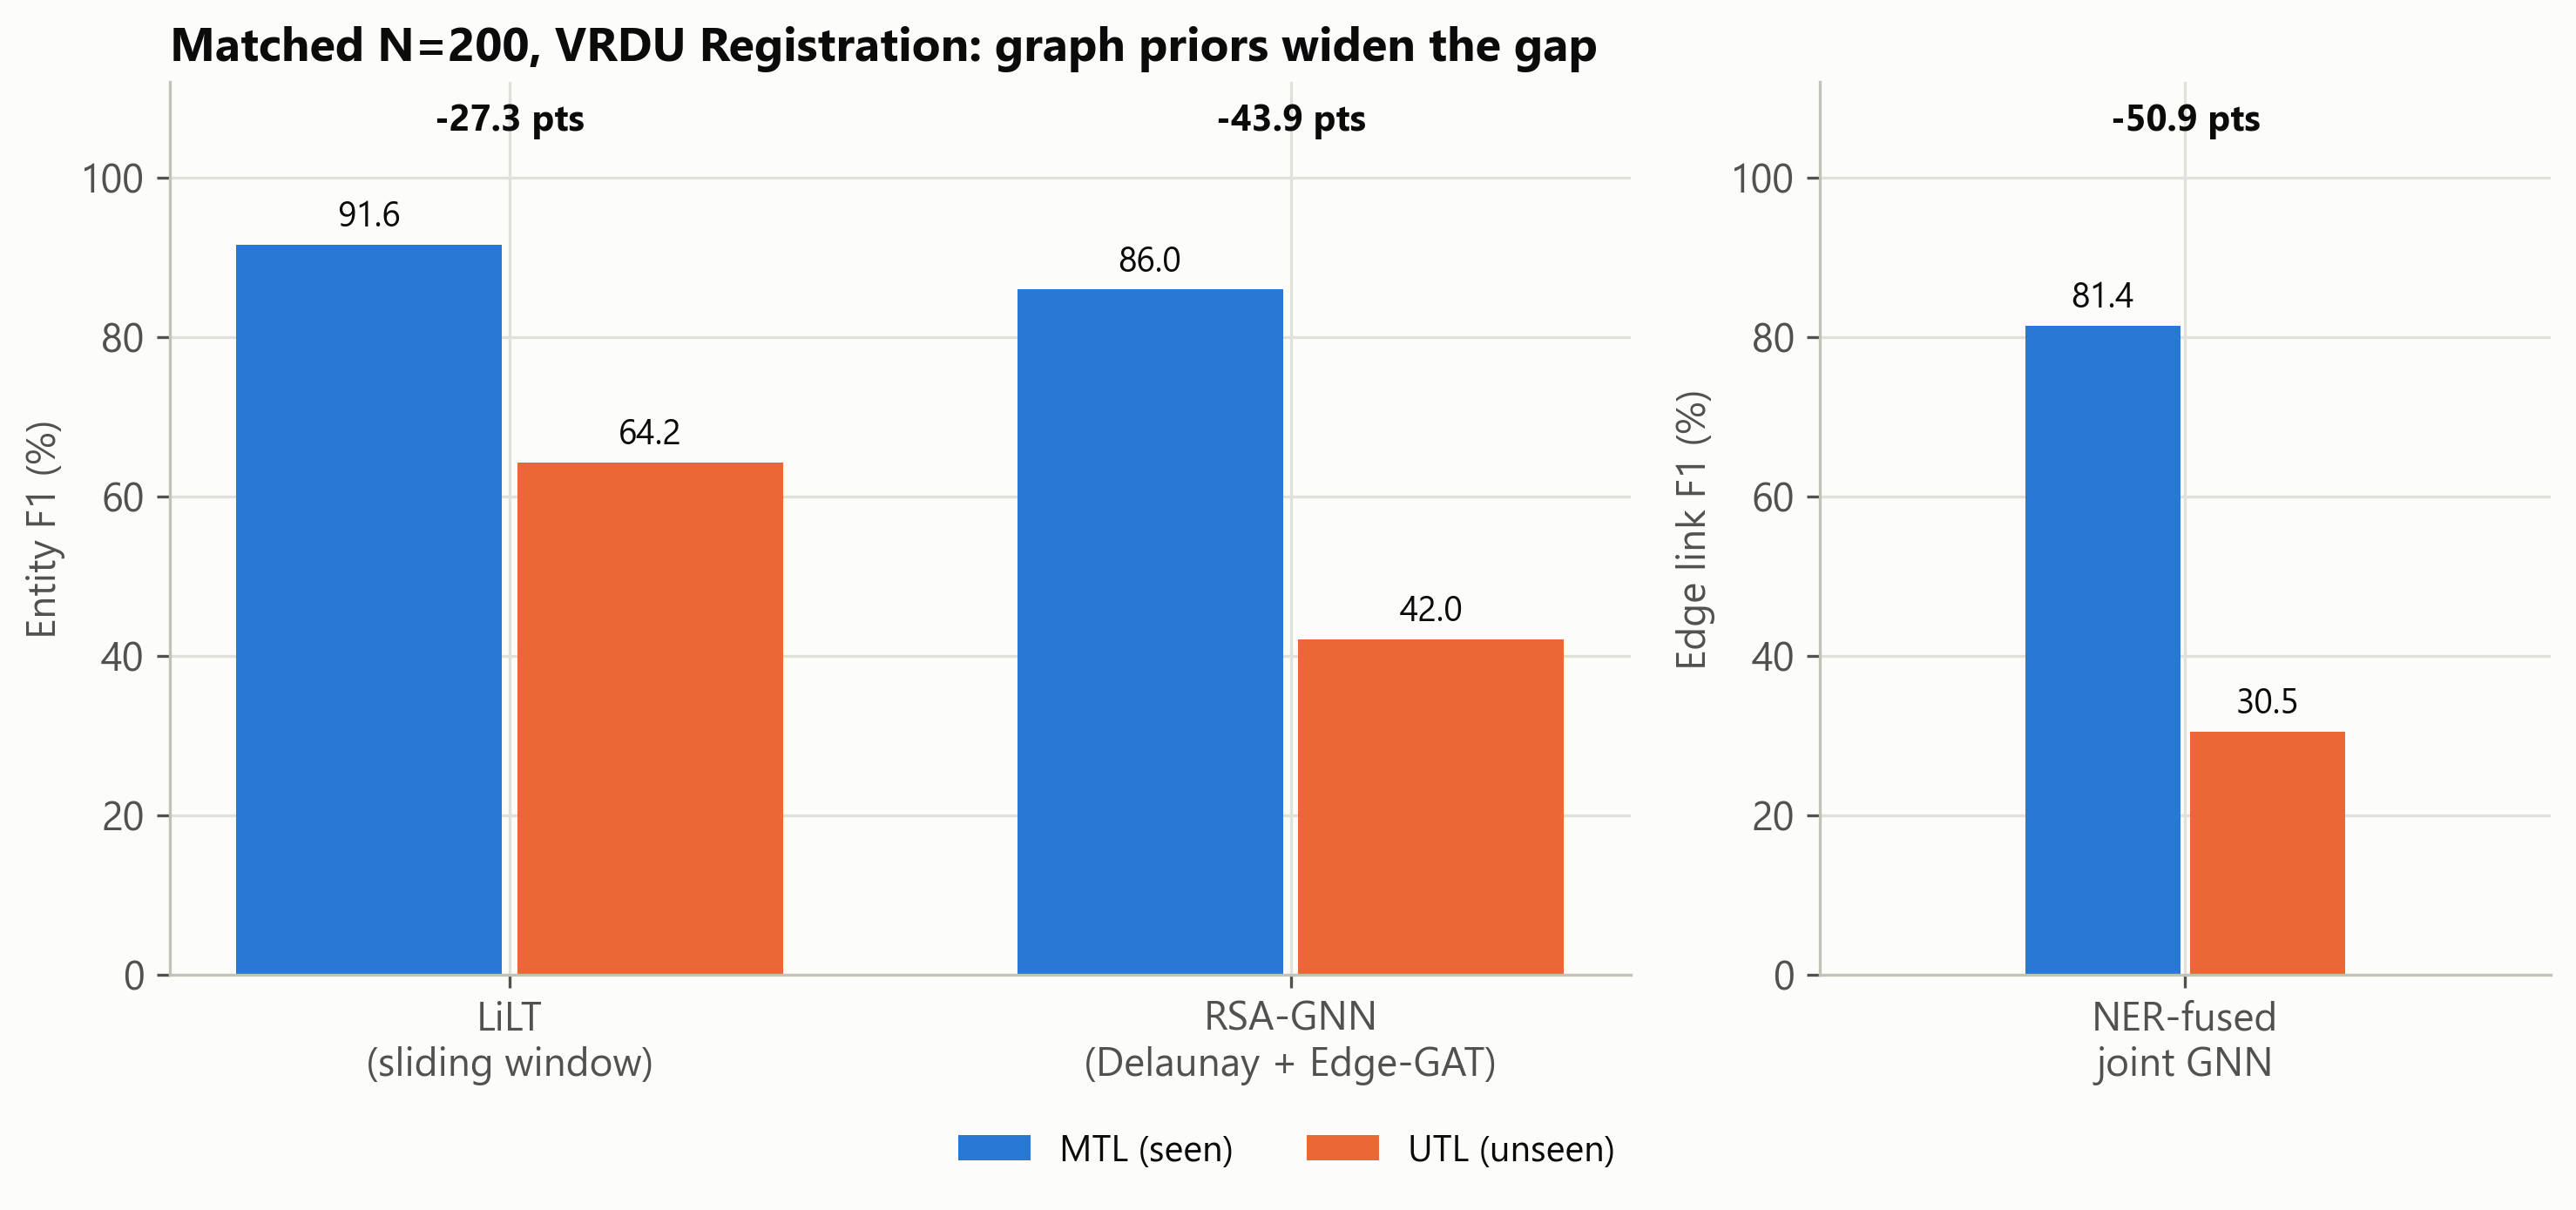
\includegraphics[width=0.58\linewidth]{fig6_gnn_utl_comparison.png}
\caption{Left: Edge-GAT ablations on a random document split (2 seeds). Right: matched-protocol comparison on registration forms; the NER-fused model reports edge link F1, so it has its own axis.}
\label{fig:gnn}
\end{figure}

On a random document split (Figure~\ref{fig:gnn}, left) the graph models are strong. Adding the 16 edge features to a plain GAT raises entity F1 from 89.01 to 89.91, and a third layer raises it to 90.50. These numbers are close to LiLT on seen templates even though the graph model only sees frozen LiLT features.

Under the matched template-disjoint protocol the picture reverses (Figure~\ref{fig:gnn}, right). RSA-GNN goes from 85.97 to 42.05 F1, a gap of 43.92 points against 27.31 for LiLT with the same windowing. The NER-fused GNN goes from 81.40 to 30.48 edge link F1, a gap of 50.92. Our hypothesis was wrong in this setting. We think the reason is that a Delaunay triangulation depends entirely on layout. When a template puts values below their keys instead of beside them, or switches to a multi-column grid, each word gets a different set of neighbours, and message passing mixes in context that the model never saw during training. The fused model adds a second layout-dependent signal, since its heuristic link labels assume the value sits to the right of or below the key. LiLT's text stream still carries meaning that does not depend on position, which is likely why it degrades less.

\subsection{Key-value linking}

\begin{table}[H]
\centering\small
\caption{Joint tagging and linking (3 seeds, standard splits).}
\label{tab:link}
\begin{tabular}{@{}lcc@{}}
\toprule
Model & Entity F1 & Linking F1 \\
\midrule
FUNSD, first joint model (10 features, BCE, no curriculum) & 79.10 $\pm$ 0.79 & 32.05 $\pm$ 2.74 \\
XFUND, 12 features + curriculum + focal + one-to-one & 79.09 $\pm$ 0.21 & 65.51 $\pm$ 1.26 \\
XFUND, full 16 features & 79.32 $\pm$ 0.36 & 67.21 $\pm$ 0.83 \\
Synthetic forms & 100.00 & 100.00 \\
\bottomrule
\end{tabular}
\end{table}

\begin{figure}[H]
\centering
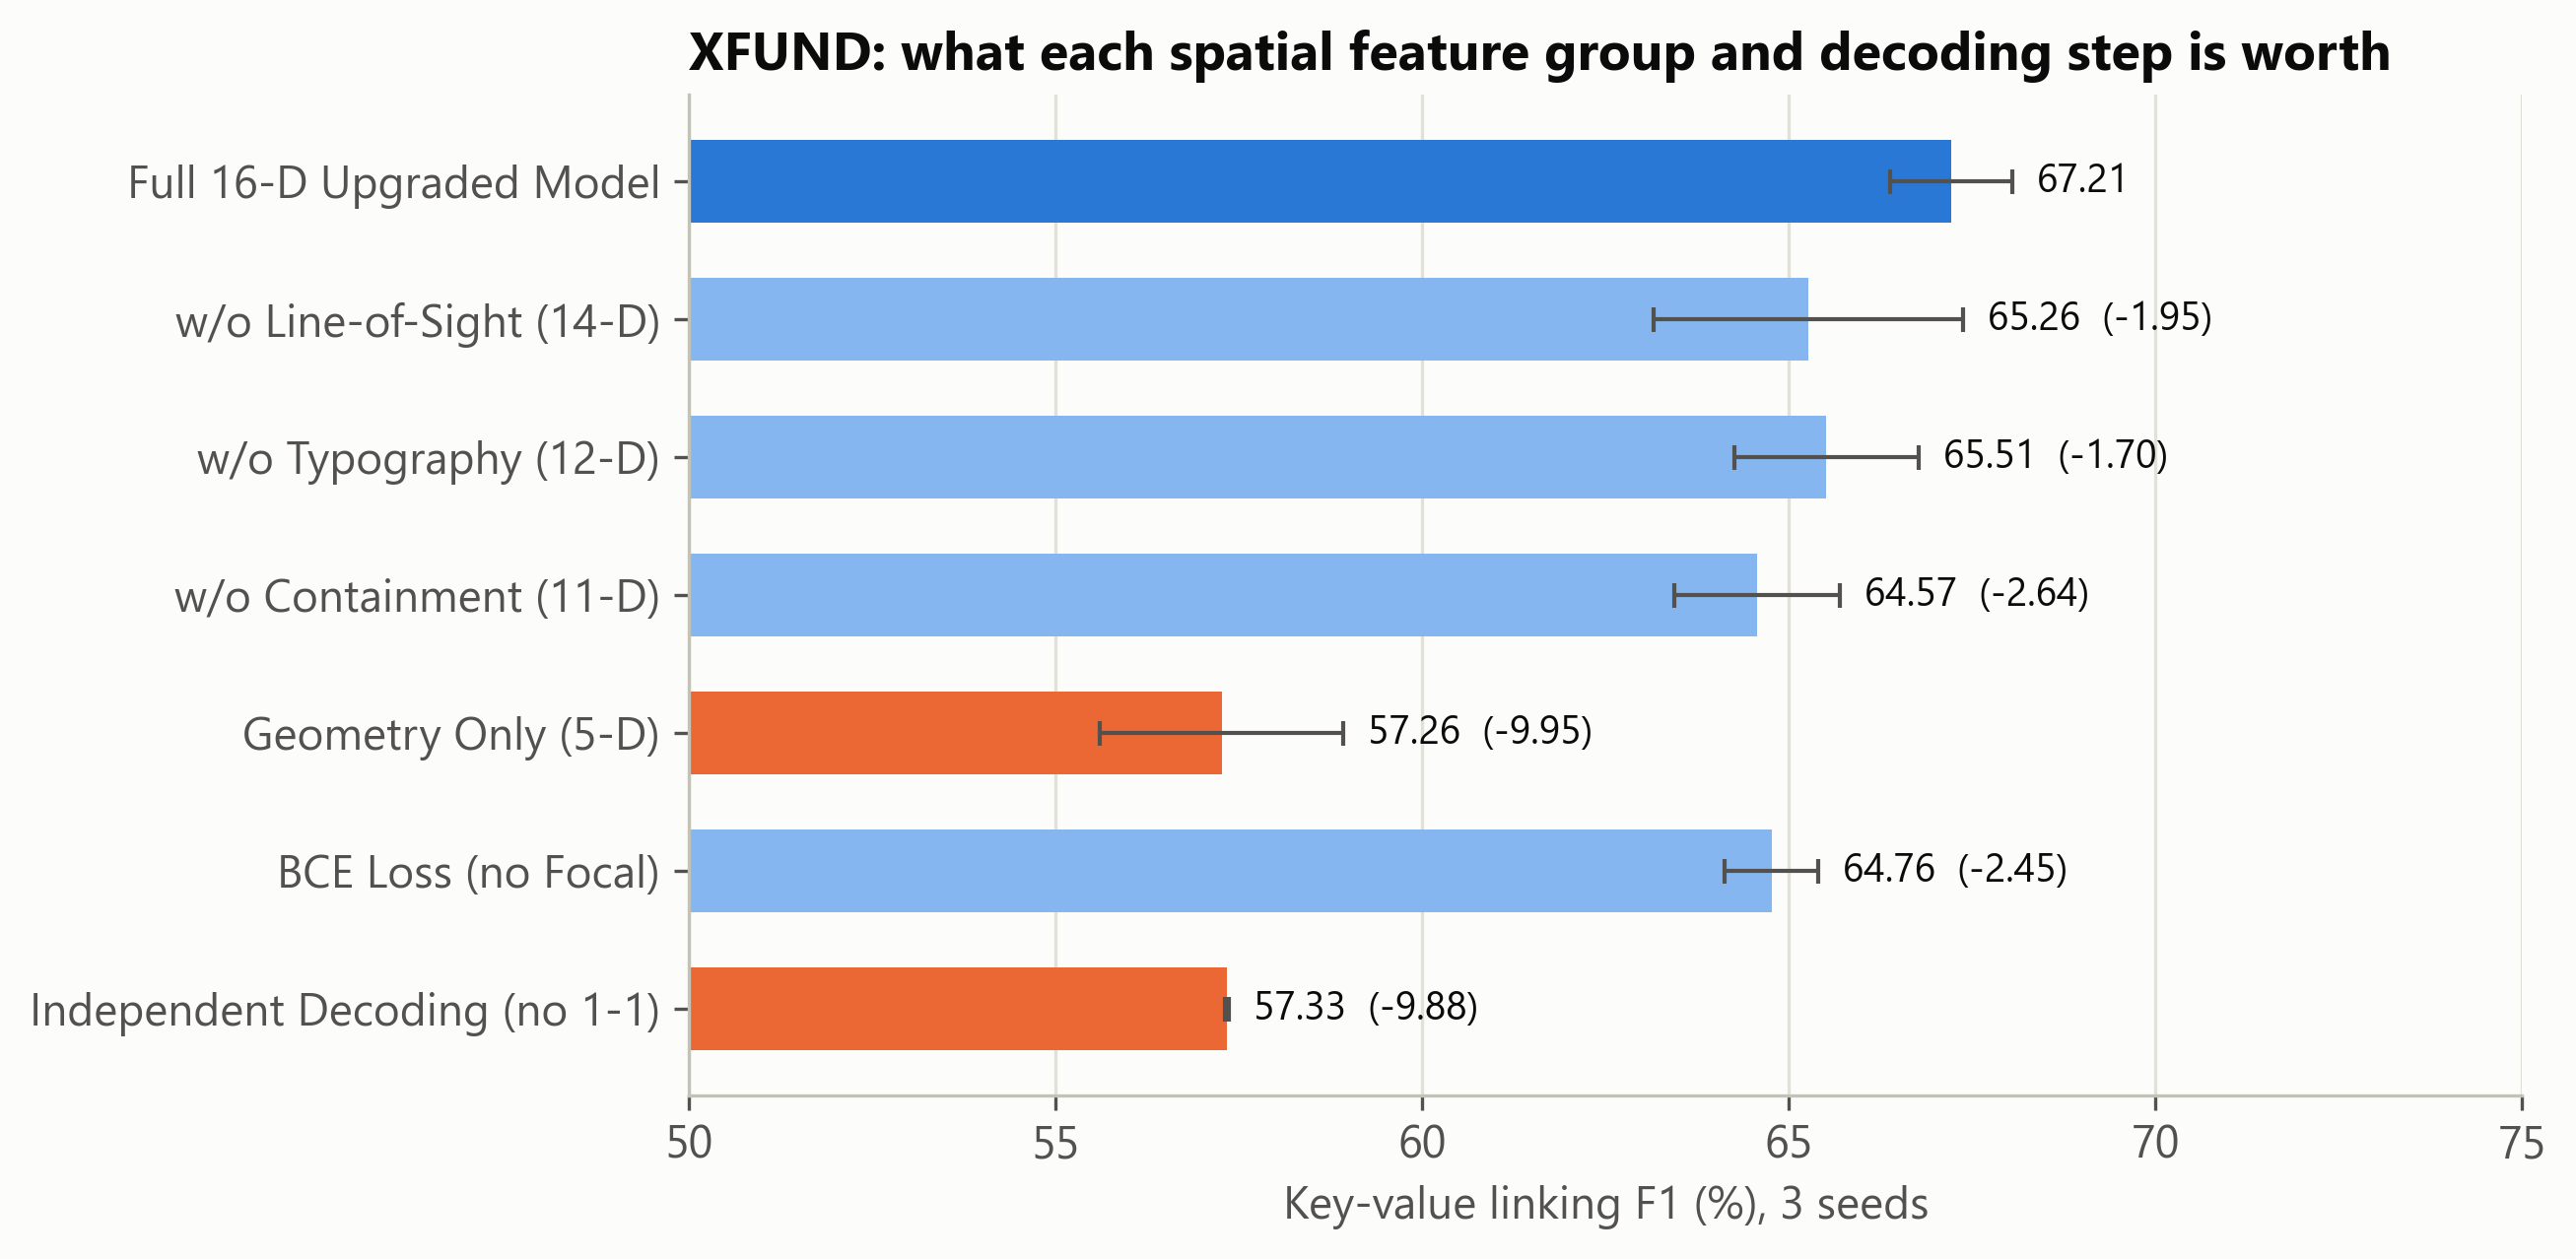
\includegraphics[width=0.78\linewidth]{fig5_xfund_knockouts.png}
\caption{XFUND linking F1 when one feature group or decoding step is removed from the full model (3 seeds).}
\label{fig:knockout}
\end{figure}

The first joint model on FUNSD predicted about three times as many links as there are (3,169 predicted against 1,031 gold in one seed), giving high recall but precision near 0.2. The changes made after the review fixed most of this. In the knockout study (Figure~\ref{fig:knockout}), one-to-one decoding is worth about 10 points: without it, linking F1 falls to 57.33. Keeping only the five geometry features costs a similar amount (57.26), so containment, line of sight and typography together carry about 10 points. Removing any one of these groups costs 1.7 to 2.6 points, and replacing focal loss with BCE costs 2.45. Entity F1 stays near 79 in every condition, so these components affect linking only. The synthetic forms are solved perfectly; they come from a train/test split over the same seven families and only show that the pipeline works end to end, not that it generalises.

% ----------------------------------------------------------------------------
\section{Interface}

We built two Gradio applications. The first (\texttt{demo.py}) accepts a PNG, JPG or PDF upload. PDFs are rendered with PyMuPDF; images go through RapidOCR to get words and boxes. Entities are labelled by heuristics that split "Key: value" lines on the colon, and by the joint LiLT model when its checkpoint is present. Keys and values are then paired by a rule-based matcher that uses horizontal and vertical line of sight, distance and a regular-expression type check, followed by greedy one-to-one assignment. The output is the page with coloured boxes and arrows, a key-value table and a JSON graph. A second tab generates a synthetic form from any of the seven families. The second application (\texttt{demo\_gnn.py}) runs the graph pipeline: OCR, Delaunay graph with ruled-line pruning on the real page image, LiLT features and the three-layer Edge-GAT, predicting the six registration fields and optionally drawing the graph over the page. \todo{add a screenshot of the running demo}

% ----------------------------------------------------------------------------
\section{Plan for Novelty Assessment}

Each item targets a failure we measured.
\begin{enumerate}
  \item \textbf{Linking on held-out templates.} We found no work that tests key-value linking on unseen templates. We plan to build such a test by holding out whole form families (from the synthetic generator and from XFUND or FUNSD clusters of similar forms) and to report linking F1 under the same matched protocol.
  \item \textbf{Template-adversarial LiLT.} Add a classifier that predicts the template from LiLT's representation and train it through a gradient-reversal layer \cite{dann}, so the encoder is pushed to drop template-specific information.
  \item \textbf{Relative 2-D attention.} Replace the absolute box embeddings with relative positions inside self-attention, in the style of BROS \cite{bros}, so that moving a whole block of the form does not change its representation.
  \item \textbf{Learned graph edges.} Let text similarity between words decide which nodes connect, instead of a fixed Delaunay triangulation.
\end{enumerate}
We will judge each idea by whether it reduces the unseen-template gap while keeping seen-template F1.

% ----------------------------------------------------------------------------
\section{Conclusion}

We set out to measure how well key-value extraction carries over to form templates a model has never seen. With a strict, matched protocol we found a 21-point gap for LiLT on VRDU registration forms and less than 2 points on the more uniform Ad-Buy forms, so the difficulty depends on how much the templates differ. The failures are concentrated in fields whose position changes between templates and whose text is not distinctive; OCR errors play almost no part, and validation on seen templates does not reveal the problem. Graph models built on a fixed geometric neighbourhood fit seen layouts well but widen the gap to 44 points, which tells us that more spatial structure is not the answer when the structure itself changes. For linking, constrained decoding and richer spatial features took XFUND linking F1 from 32 to 67. These results point to our next step: representations that are explicitly discouraged from encoding the template, evaluated on linking as well as tagging.

% ----------------------------------------------------------------------------
\begin{thebibliography}{99}
\small

\bibitem{vrdu} Zilong Wang, Yichao Zhou, Wei Wei, Chen-Yu Lee and Sandeep Tata. VRDU: A Benchmark for Visually-rich Document Understanding, KDD, 2023. \url{https://arxiv.org/abs/2211.15421}

\bibitem{funsd} Guillaume Jaume, Hazim Kemal Ekenel and Jean-Philippe Thiran. FUNSD: A Dataset for Form Understanding in Noisy Scanned Documents, ICDAR-OST, 2019. \url{https://arxiv.org/abs/1905.13538}

\bibitem{xfund} Yiheng Xu, Tengchao Lv, Lei Cui, Guoxin Wang, Yijuan Lu, Dinei Florencio, Cha Zhang and Furu Wei. XFUND: A Benchmark Dataset for Multilingual Visually Rich Form Understanding, Findings of ACL, 2022. \url{https://aclanthology.org/2022.findings-acl.253/}

\bibitem{layoutlm} Yiheng Xu, Minghao Li, Lei Cui, Shaohan Huang, Furu Wei and Ming Zhou. LayoutLM: Pre-training of Text and Layout for Document Image Understanding, KDD, 2020. \url{https://arxiv.org/abs/1912.13318}

\bibitem{layoutlmv3} Yupan Huang, Tengchao Lv, Lei Cui, Yutong Lu and Furu Wei. LayoutLMv3: Pre-training for Document AI with Unified Text and Image Masking, ACM Multimedia, 2022. \url{https://arxiv.org/abs/2204.08387}

\bibitem{lilt} Jiapeng Wang, Lianwen Jin and Kai Ding. LiLT: A Simple yet Effective Language-Independent Layout Transformer for Structured Document Understanding, ACL, 2022. \url{https://arxiv.org/abs/2202.13669}

\bibitem{bros} Teakgyu Hong, Donghyun Kim, Mingi Ji, Wonseok Hwang, Daehyun Nam and Sungrae Park. BROS: A Pre-trained Language Model Focusing on Text and Layout for Better Key Information Extraction from Documents, AAAI, 2022. \url{https://arxiv.org/abs/2108.04539}

\bibitem{formnet} Chen-Yu Lee, Chun-Liang Li, Timothy Dozat, Vincent Perot, Guolong Su, Nan Hua, Joshua Ainslie, Renshen Wang, Yasuhisa Fujii and Tomas Pfister. FormNet: Structural Encoding beyond Sequential Modeling in Form Document Information Extraction, ACL, 2022. \url{https://arxiv.org/abs/2203.08411}

\bibitem{geolayoutlm} Chuwei Luo, Changxu Cheng, Qi Zheng and Cong Yao. GeoLayoutLM: Geometric Pre-training for Visual Information Extraction, CVPR, 2023. \url{https://arxiv.org/abs/2304.10759}

\bibitem{doc2graph} Andrea Gemelli, Sanket Biswas, Enrico Civitelli, Josep Llad\'os and Simone Marinai. Doc2Graph: A Task Agnostic Document Understanding Framework Based on Graph Neural Networks, ECCV Workshops, 2022. \url{https://arxiv.org/abs/2208.11168}

\bibitem{gat} Petar Veli\v{c}kovi\'c, Guillem Cucurull, Arantxa Casanova, Adriana Romero, Pietro Li\`o and Yoshua Bengio. Graph Attention Networks, ICLR, 2018. \url{https://arxiv.org/abs/1710.10903}

\bibitem{biaffine} Timothy Dozat and Christopher D. Manning. Deep Biaffine Attention for Neural Dependency Parsing, ICLR, 2017. \url{https://arxiv.org/abs/1611.01734}

\bibitem{focal} Tsung-Yi Lin, Priya Goyal, Ross Girshick, Kaiming He and Piotr Doll\'ar. Focal Loss for Dense Object Detection, ICCV, 2017. \url{https://arxiv.org/abs/1708.02002}

\bibitem{dann} Yaroslav Ganin, Evgeniya Ustinova, Hana Ajakan, Pascal Germain, Hugo Larochelle, Fran\c{c}ois Laviolette, Mario Marchand and Victor Lempitsky. Domain-Adversarial Training of Neural Networks, JMLR, 2016. \url{https://arxiv.org/abs/1505.07818}

\bibitem{augraphy} Alexander Groleau, Kok Wei Chee, Stefan Larson, Samay Maini and Jonathan Boarman. Augraphy: A Data Augmentation Library for Document Images, ICDAR, 2023. \url{https://arxiv.org/abs/2208.14558}

\bibitem{vrdurepo} Google Research. \url{https://github.com/google-research-datasets/vrdu}, Accessed on: 19th September, 2026.

\bibitem{funsdsite} Guillaume Jaume. \url{https://guillaumejaume.github.io/FUNSD/}, Accessed on: 19th September, 2026.

\bibitem{xfundrepo} Microsoft (doc-analysis). \url{https://github.com/doc-analysis/XFUND}, Accessed on: 14th October, 2026.

\bibitem{liltckpt} SCUT-DLVCLab. \url{https://huggingface.co/SCUT-DLVCLab/lilt-roberta-en-base}, Accessed on: 19th September, 2026.

\bibitem{ourrepo} Arjoe Basak and Param Mehta. \url{https://github.com/ABasakEE/KeyValue-Extraction}, Accessed on: 26th October, 2026.

\end{thebibliography}

\end{document}
